%  LaTeX support: latex@mdpi.com 
%  In case you need support, please attach all files that are necessary for compiling as well as the log file, and specify the details of your LaTeX setup (which operating system and LaTeX version / tools you are using).

%=================================================================
\documentclass[preprints,article,accept,moreauthors,pdftex]{Definitions/mdpi} 
%\documentclass[aerospace,article,submit,moreauthors,pdftex]{Definitions/mdpi} 

% If you would like to post an early version of this manuscript as a preprint, you may use preprint as the journal and change 'submit' to 'accept'. The document class line would be, e.g., \documentclass[preprints,article,accept,moreauthors,pdftex]{mdpi}. This is especially recommended for submission to arXiv, where line numbers should be removed before posting. For preprints.org, the editorial staff will make this change immediately prior to posting.

%%%%%%%%%%%%%%%%%%%%%%%%%%%%%%%%%%%%%%%%%%%%%%%%%%%%%%%%%%
%% additional packages
\usepackage[printonlyused]{acronym}
\usepackage{comment}
% avoid acronym links
\makeatletter
\AtBeginDocument{%
  \renewcommand*{\AC@hyperlink}[2]{%
    \begingroup
      \hypersetup{hidelinks}%
      \hyperlink{#1}{#2}%
    \endgroup
  }%
}
\makeatother

% acrolist line spacing
\usepackage{xpatch}
\makeatletter
\xpatchcmd{\AC@deflist}
  {\addtolength{\leftmargin}{\labelsep}}
  {\addtolength{\leftmargin}{\labelsep}\setlength{\itemsep}{10pt}}
  {}{}
\makeatother

% comments
\newcommand{\Jakob}[1]{{{\color{orange}{\itshape{#1}}\color{black}}
    }{\ignorespaces}}
    
% subfigures
\usepackage{caption}
\usepackage{subcaption}
%%%%%%%%%%%%%%%%%%%%%%%%%%%%%%%%%%%%%%%%%%%%%%%%%%%%%%%%%%


%--------------------
% Class Options:
%--------------------
%----------
% journal
%----------
% Choose between the following MDPI journals:
% acoustics, actuators, addictions, admsci, aerospace, agriculture, agriengineering, agronomy, algorithms, animals, antibiotics, antibodies, antioxidants, applsci, arts, asc, asi, atmosphere, atoms, axioms, batteries, bdcc, behavsci , beverages, bioengineering, biology, biomedicines, biomimetics, biomolecules, biosensors, brainsci , buildings, cancers, carbon , catalysts, cells, ceramics, challenges, chemengineering, chemistry, chemosensors, children, cleantechnol, climate, clockssleep, cmd, coatings, colloids, computation, computers, condensedmatter, cosmetics, cryptography, crystals, dairy, data, dentistry, designs , diagnostics, diseases, diversity, drones, econometrics, economies, education, ejihpe, electrochem, electronics, energies, entropy, environments, epigenomes, est, fermentation, fibers, fire, fishes, fluids, foods, forecasting, forests, fractalfract, futureinternet, futurephys, galaxies, games, gastrointestdisord, gels, genealogy, genes, geohazards, geosciences, geriatrics, hazardousmatters, healthcare, heritage, highthroughput, horticulturae, humanities, hydrology, ijerph, ijfs, ijgi, ijms, ijns, ijtpp, informatics, information, infrastructures, inorganics, insects, instruments, inventions, iot, j, jcdd, jcm, jcp, jcs, jdb, jfb, jfmk, jimaging, jintelligence, jlpea, jmmp, jmse, jnt, jof, joitmc, jpm, jrfm, jsan, land, languages, laws, life, literature, logistics, lubricants, machines, magnetochemistry, make, marinedrugs, materials, mathematics, mca, medicina, medicines, medsci, membranes, metabolites, metals, microarrays, micromachines, microorganisms, minerals, modelling, molbank, molecules, mps, mti, nanomaterials, ncrna, neuroglia, nitrogen, notspecified, nutrients, ohbm, optics, particles, pathogens, pharmaceuticals, pharmaceutics, pharmacy, philosophies, photonics, physics, plants, plasma, polymers, polysaccharides, preprints , proceedings, processes, proteomes, psych, publications, quantumrep, quaternary, qubs, reactions, recycling, religions, remotesensing, reports, resources, risks, robotics, safety, sci, scipharm, sensors, separations, sexes, signals, sinusitis, smartcities, sna, societies, socsci, soilsystems, sports, standards, stats, surfaces, surgeries, sustainability, symmetry, systems, technologies, test, toxics, toxins, tropicalmed, universe, urbansci, vaccines, vehicles, vetsci, vibration, viruses, vision, water, wem, wevj

%---------
% article
%---------
% The default type of manuscript is "article", but can be replaced by: 
% abstract, addendum, article, benchmark, book, bookreview, briefreport, casereport, changes, comment, commentary, communication, conceptpaper, conferenceproceedings, correction, conferencereport, expressionofconcern, extendedabstract, meetingreport, creative, datadescriptor, discussion, editorial, essay, erratum, hypothesis, interestingimages, letter, meetingreport, newbookreceived, obituary, opinion, projectreport, reply, retraction, review, perspective, protocol, shortnote, supfile, technicalnote, viewpoint
% supfile = supplementary materials

%----------
% submit
%----------
% The class option "submit" will be changed to "accept" by the Editorial Office when the paper is accepted. This will only make changes to the frontpage (e.g., the logo of the journal will get visible), the headings, and the copyright information. Also, line numbering will be removed. Journal info and pagination for accepted papers will also be assigned by the Editorial Office.

%------------------
% moreauthors
%------------------
% If there is only one author the class option oneauthor should be used. Otherwise use the class option moreauthors.

%---------
% pdftex
%---------
% The option pdftex is for use with pdfLaTeX. If eps figures are used, remove the option pdftex and use LaTeX and dvi2pdf.

%=================================================================
\firstpage{1} 
\makeatletter 
\setcounter{page}{\@firstpage} 
\makeatother
\pubvolume{xx}
\issuenum{1}
\articlenumber{5}
\pubyear{2019}
\copyrightyear{2019}
%\externaleditor{Academic Editor: name}
\history{Received: date; Accepted: date; Published: date}
%\updates{yes} % If there is an update available, un-comment this line

%% MDPI internal command: uncomment if new journal that already uses continuous page numbers 
%\continuouspages{yes}

%------------------------------------------------------------------
% The following line should be uncommented if the LaTeX file is uploaded to arXiv.org
%\pdfoutput=1

%=================================================================
% Add packages and commands here. The following packages are loaded in our class file: fontenc, calc, indentfirst, fancyhdr, graphicx, lastpage, ifthen, lineno, float, amsmath, setspace, enumitem, mathpazo, booktabs, titlesec, etoolbox, amsthm, hyphenat, natbib, hyperref, footmisc, geometry, caption, url, mdframed, tabto, soul, multirow, microtype, tikz

%=================================================================
%% Please use the following mathematics environments: Theorem, Lemma, Corollary, Proposition, Characterization, Property, Problem, Example, ExamplesandDefinitions, Hypothesis, Remark, Definition, Notation, Assumption
%% For proofs, please use the proof environment (the amsthm package is loaded by the MDPI class).

%=================================================================
% Full title of the paper (Capitalized)
\Title{Design Space Exploration of a Turbojet Part using a Combined Object Model for Function and Geometry}

% Author Orchid ID: enter ID or remove command
\newcommand{\orcidauthorA}{0000-0002-2270-6253} % Add \orcidA{} behind the author's name
\newcommand{\orcidauthorB}{0000-0001-5216-0944} % Add \orcidB{} behind the author's name
\newcommand{\orcidauthorC}{0000-0003-0373-3720} % Add \orcidC{} behind the author's name

% Authors, for the paper (add full first names)
\Author{Jakob R. Müller $^{1}$*\orcidA{}, Massimo Panarotto $^{1}$\orcidB{} and Ola Isaksson $^{1,}$\orcidC{}}

% Authors, for metadata in PDF
\AuthorNames{Jakob R. Müller, Massimo Panarotto and Ola Isaksson}

% Affiliations / Addresses (Add [1] after \address if there is only one affiliation.)
\address{%
$^{1}$ \quad Chalmers University of Technology, Gothenburg}

% Contact information of the corresponding author
\corres{Correspondence: jakob.muller@chalmers.se}

% Current address and/or shared authorship
%\firstnote{Current address: Affiliation 3} 
%\secondnote{These authors contributed equally to this work.}
% The commands \thirdnote{} till \eighthnote{} are available for further notes

%\simplesumm{} % Simple summary

%\conference{} % An extended version of a conference paper

% Abstract (Do not insert blank lines, i.e. \\) 
\abstract{Product development, especially in the development of aerospace components, hinges on the use of CAD models and the subsequent geometry-based analyses for evaluation of the quality of a concept.
However, the generation (and variation) of a CAD model to include radical or novel design solutions is an expensive modelling effort.
To support this a combined function and geometry modelling approach, enabling the automated
generation of CAD models of variant concepts, is proposed and developed. The approach is used in the conceptual development phase of a part for a turbofan engine - an outlet guide vane (OGV) - in collaboration with an aerospace manufacturer.
The approach is tested through workshops, in which industrial practitioner interact with a tool that embeds the presented approach for function and geometry modelling. 
The practitioners used the approach to explore novel solutions and configurations. 
The evaluation activities with the industrial practitioners through interviews and questionnaires point to the potential of the approach in terms of 
1) ability to provide clear and explicit  illustration of the design rationale of the product 
2) ability to capture, integrate and model novel solutions and 
3) ability to provide a clear connection between the abstract functional and the concrete geometrical domain, which has the potential to foster innovation.
}

% Keywords
\keyword{Product development process, Design space exploration, Function modelling, CAD, Aerospace}

% The fields PACS, MSC, and JEL may be left empty or commented out if not applicable
%\PACS{J0101}
%\MSC{}
%\JEL{}

%%%%%%%%%%%%%%%%%%%%%%%%%%%%%%%%%%%%%%%%%%
% Only for the journal Diversity
%\LSID{\url{http://}}

%%%%%%%%%%%%%%%%%%%%%%%%%%%%%%%%%%%%%%%%%%
% Only for the journal Applied Sciences:
%\featuredapplication{Authors are encouraged to provide a concise description of the specific application or a potential application of the work. This section is not mandatory.}
%%%%%%%%%%%%%%%%%%%%%%%%%%%%%%%%%%%%%%%%%%

%%%%%%%%%%%%%%%%%%%%%%%%%%%%%%%%%%%%%%%%%%
% Only for the journal Data:
%\dataset{DOI number or link to the deposited data set in cases where the data set is published or set to be published separately. If the data set is submitted and will be published as a supplement to this paper in the journal Data, this field will be filled by the editors of the journal. In this case, please make sure to submit the data set as a supplement when entering your manuscript into our manuscript editorial system.}

%\datasetlicense{license under which the data set is made available (CC0, CC-BY, CC-BY-SA, CC-BY-NC, etc.)}

%%%%%%%%%%%%%%%%%%%%%%%%%%%%%%%%%%%%%%%%%%
% Only for the journal Toxins
%\keycontribution{The breakthroughs or highlights of the manuscript. Authors can write one or two sentences to describe the most important part of the paper.}

%\setcounter{secnumdepth}{4}
%%%%%%%%%%%%%%%%%%%%%%%%%%%%%%%%%%%%%%%%%%
\begin{document}
%%%%%%%%%%%%%%%%%%%%%%%%%%%%%%%%%%%%%%%%%%

% %%%%%%%%%%%%%%%%%%%%%%%%%%%%%%%%%%%%%%%%%%
% \setcounter{section}{-1} %% Remove this when starting to work on the template.
% \section{How to Use this Template}
% The template details the sections that can be used in a manuscript. Note that the order and names of article sections may differ from the requirements of the journal (e.g., the positioning of the Materials and Methods section). Please check the instructions for authors page of the journal to verify the correct order and names. For any questions, please contact the editorial office of the journal or support@mdpi.com. For LaTeX related questions please contact latex@mdpi.com.
% %The order of the section titles is: Introduction, Materials and Methods, Results, Discussion, Conclusions for these journals: aerospace,algorithms,antibodies,antioxidants,atmosphere,axioms,biomedicines,carbon,crystals,designs,diagnostics,environments,fermentation,fluids,forests,fractalfract,informatics,information,inventions,jfmk,jrfm,lubricants,neonatalscreening,neuroglia,particles,pharmaceutics,polymers,processes,technologies,viruses,vision

\section{Introduction}
The development of new aerospace components often relies on an improvement and refinement of an existing "legacy design".
However, due to rising challenges in terms of regulation and environmental requirements \cite{ACARE2017StrategicAgenda}, there is a need to explore and evaluate more radical design concepts, both on engine level \cite{Filipenko2020ComparativeSystems, Parker2010GreenEnvironment} and component level \cite{Sjunnesson2019}. 
Also, manufactures are interested to introduce new functions in their products in order to maintain competitiveness in the market. 

% need for DSE
To be able to develop novel products outside the already known design space, developers need reliable methods and tools that support them in the generation of concepts and models as well as their analysis and evaluation \cite{Woodbury2006, Kang2011, Isaksson2016}.
% currently available tools insufficient
Currently available -- and applied -- methods such as parameterisation \citep{VanDerLaan2005ParametricAnalysis} or \ac{KBE} \cite{Sandberg2011} cover only a dimensional variation of existing concepts or require an expensive setup of a master model.
Therefore, these geometry based approaches only allow for the exploration of a subset of the available design space \citep{Woodbury2006, Muller2019ICED}.
To enable a systematic, wide and efficient design space exploration \ac{DSE}, an approach connecting function and geometry models - enabling enabling the automated
generation of CAD models of variant concepts - has been recently developed.
The approach is called \textit{\acf{FGE}}  \cite{Muller2021FunctionVariants}.
The approach aims to enable a parallel development approach in both, the functional and geometrical, domains.
This can enable product developers to associate the geometry directly with the function it fulfils and vice versa, investigate into novel concepts and analyse them.
% Therefore, new solutions can be integrated for specific functional requirements, while allowing to only alter the related geometry and observing the impact of the alteration onto the product as a system.
% Furthermore does the approach allow to trace changes in requirements and functions onto the product's geometry, enabling a more precise redesign process in the case of requirement changes.

% paper overview
This publication reports from an qualitative study about the application of the \ac{FGE} approach in a development project for a static turbine structure, a fan frame \ac{OGV}. 
The study has been conducted in collaboration with an aerospace manufacturer. 
The study investigates into whether the proposed method does \textit{improve \ac{DSE}} in that it enables the \textit{capture}, \textit{representation} and \textit{embodiment} of novel design concepts.

%Section \ref{sec:background} explains the relevant technologies which the approach is build or that are comparable in functionality.
How the study has been setup and how the approach has been evaluated is explained in Section \ref{sec:method}.
The \ac{FGE} approach itself is shortly explained in Section \ref{sec:omfgDSE}, while the application of it in the industrial setting in Section \ref{sec:results}. 
The practitioners' evaluation and reflections on the application of the approach on the industrial use case  are presented in Section \ref{sec:feedback}.
Section \ref{sec:discussion} discusses these results in relation to the problematic described above as well as compared to similar approaches.
Lastly, section \ref{sec:conclusions} summarises the contribution of this paper and proposes further development of the approach.


% \Jakob{Problem: DSE is too minimal in its current form. 

% Current form = legacy design, hard focus on evolutionary development of CAD model, EWB (MDA approach for DSE), parameterisation of CAD

% proposed approach: omfgDSE

% criteria:
% }

% \subsection{Design space exploration}
% The design space is the sum of all possible concepts which fulfil the requirements \cite{Saxena2010}.
% However, the number of concepts is neigh infinite \cite{Woodbury2006}, and therefor it is not possible to explore all of them.

% To \textit{explore} means in this case to generate product concept descriptions which presumably reside inside the design space -- that is, fulfil all requirements and functions -- and analyse it for its performance.
% The analysis has two-fold aim: first, to verify whether the concept actually does fulfil all requirements, and second how well it does, to be able to compare it with other designs and chose the best available.
% The concept descriptions required for this are in most cases -- especially in the aerospace industry -- CAD models \cite{}.
% These models are used for subsequent product behaviour analysis such as aerodynamic, structural or thermodynamic simulations.

% In most cases, the design space is explored by varying an existing \textit{legacy model}, and generating variants of it \cite{Prasad2006}.
% This approach, mainly building on engineers' experience and 

% \subsection{Function modelling}

% \Jakob{
% KBE: \citep{LaRocca2012}; parametric design \citep{vanderlaan2005}

% FBS \citep{Gero2004}; 

% EF-M \citep{Schachinger2000}, 

% geometric feature based modelling \citep{}, 

% }
 

% \subsection{Design automation}


%%%%%%%%%%%%%%%%%%%%%%%%%%%%%%%%%%%%%%%%%%%%%%%%%%%%%%%%%%%%%%%%%%%%%%%%%%%%%%%%%%%%%%%%%%%%%%%%%%%%%%%
\subsection{The FGE approach}\label{sec:omfgDSE}
% EF-M
The \acf{FGE} approach builds on the function modelling method \ac{EF-M} and combines it with a \ac{DA} approach based on \acp{UDF}, realised in the CAD software Siemens NX. 
One main assumption behind the approach is that every geometrical element in a product has a specific function \citep{Gero2004}.
This function can be identified, and the geometry can be isolated.
As a result, these two information sets can be coupled. 
The other main assumption for the approach is that if the function of a geometry element is identified, alternative solutions for that function  

As an example (Figure \ref{fig:decompositionExample}), two functions in an \ac{OGV} are "connect vane to fitting" solved by "glue" and "interface to front centre body" solved by "barrel nuts", such \ac{DS} are associated to geometry elements, as shown in the figure.    

\begin{figure}[ht]
    \centering
    \includegraphics[width=.6\textwidth]{figures/ogvInitialDecompGeo.png}
    \caption{Example of function and design solutions of an OGV, connected to geometry elements.
    The different geometry elements are colour coded to show their extend.}
    \label{fig:decompositionExample}
\end{figure}

To enable the capture of a product's functional architecture, \ac{EF-M} modelling has been selected. 
The reason for this ability of \ac{EF-M} to represent the design space through functions and constraints, capture and represent alternative solutions on any abstraction level and the option for first-level analysis based purely on a function model \cite{Muller2019Aiedam}.
The function model is created by alternating \ac{FR} and their respective \ac{DS} in a tree like structure \cite{Schachinger2000}.
Since \ac{EF-M} follows the axiom of independence of Suh's axiomatic design \cite{Suh1990}, each \ac{FR} is -- in one concept -- solved by \textit{only one} \ac{DS}. 
If there are more \ac{DS} per \ac{FR} modelled, these represent alternatives.
This is illustrated in \ref{fig:EFM} in the form of "Solution A" and "Solution B".

\begin{figure}[ht]
    \centering
    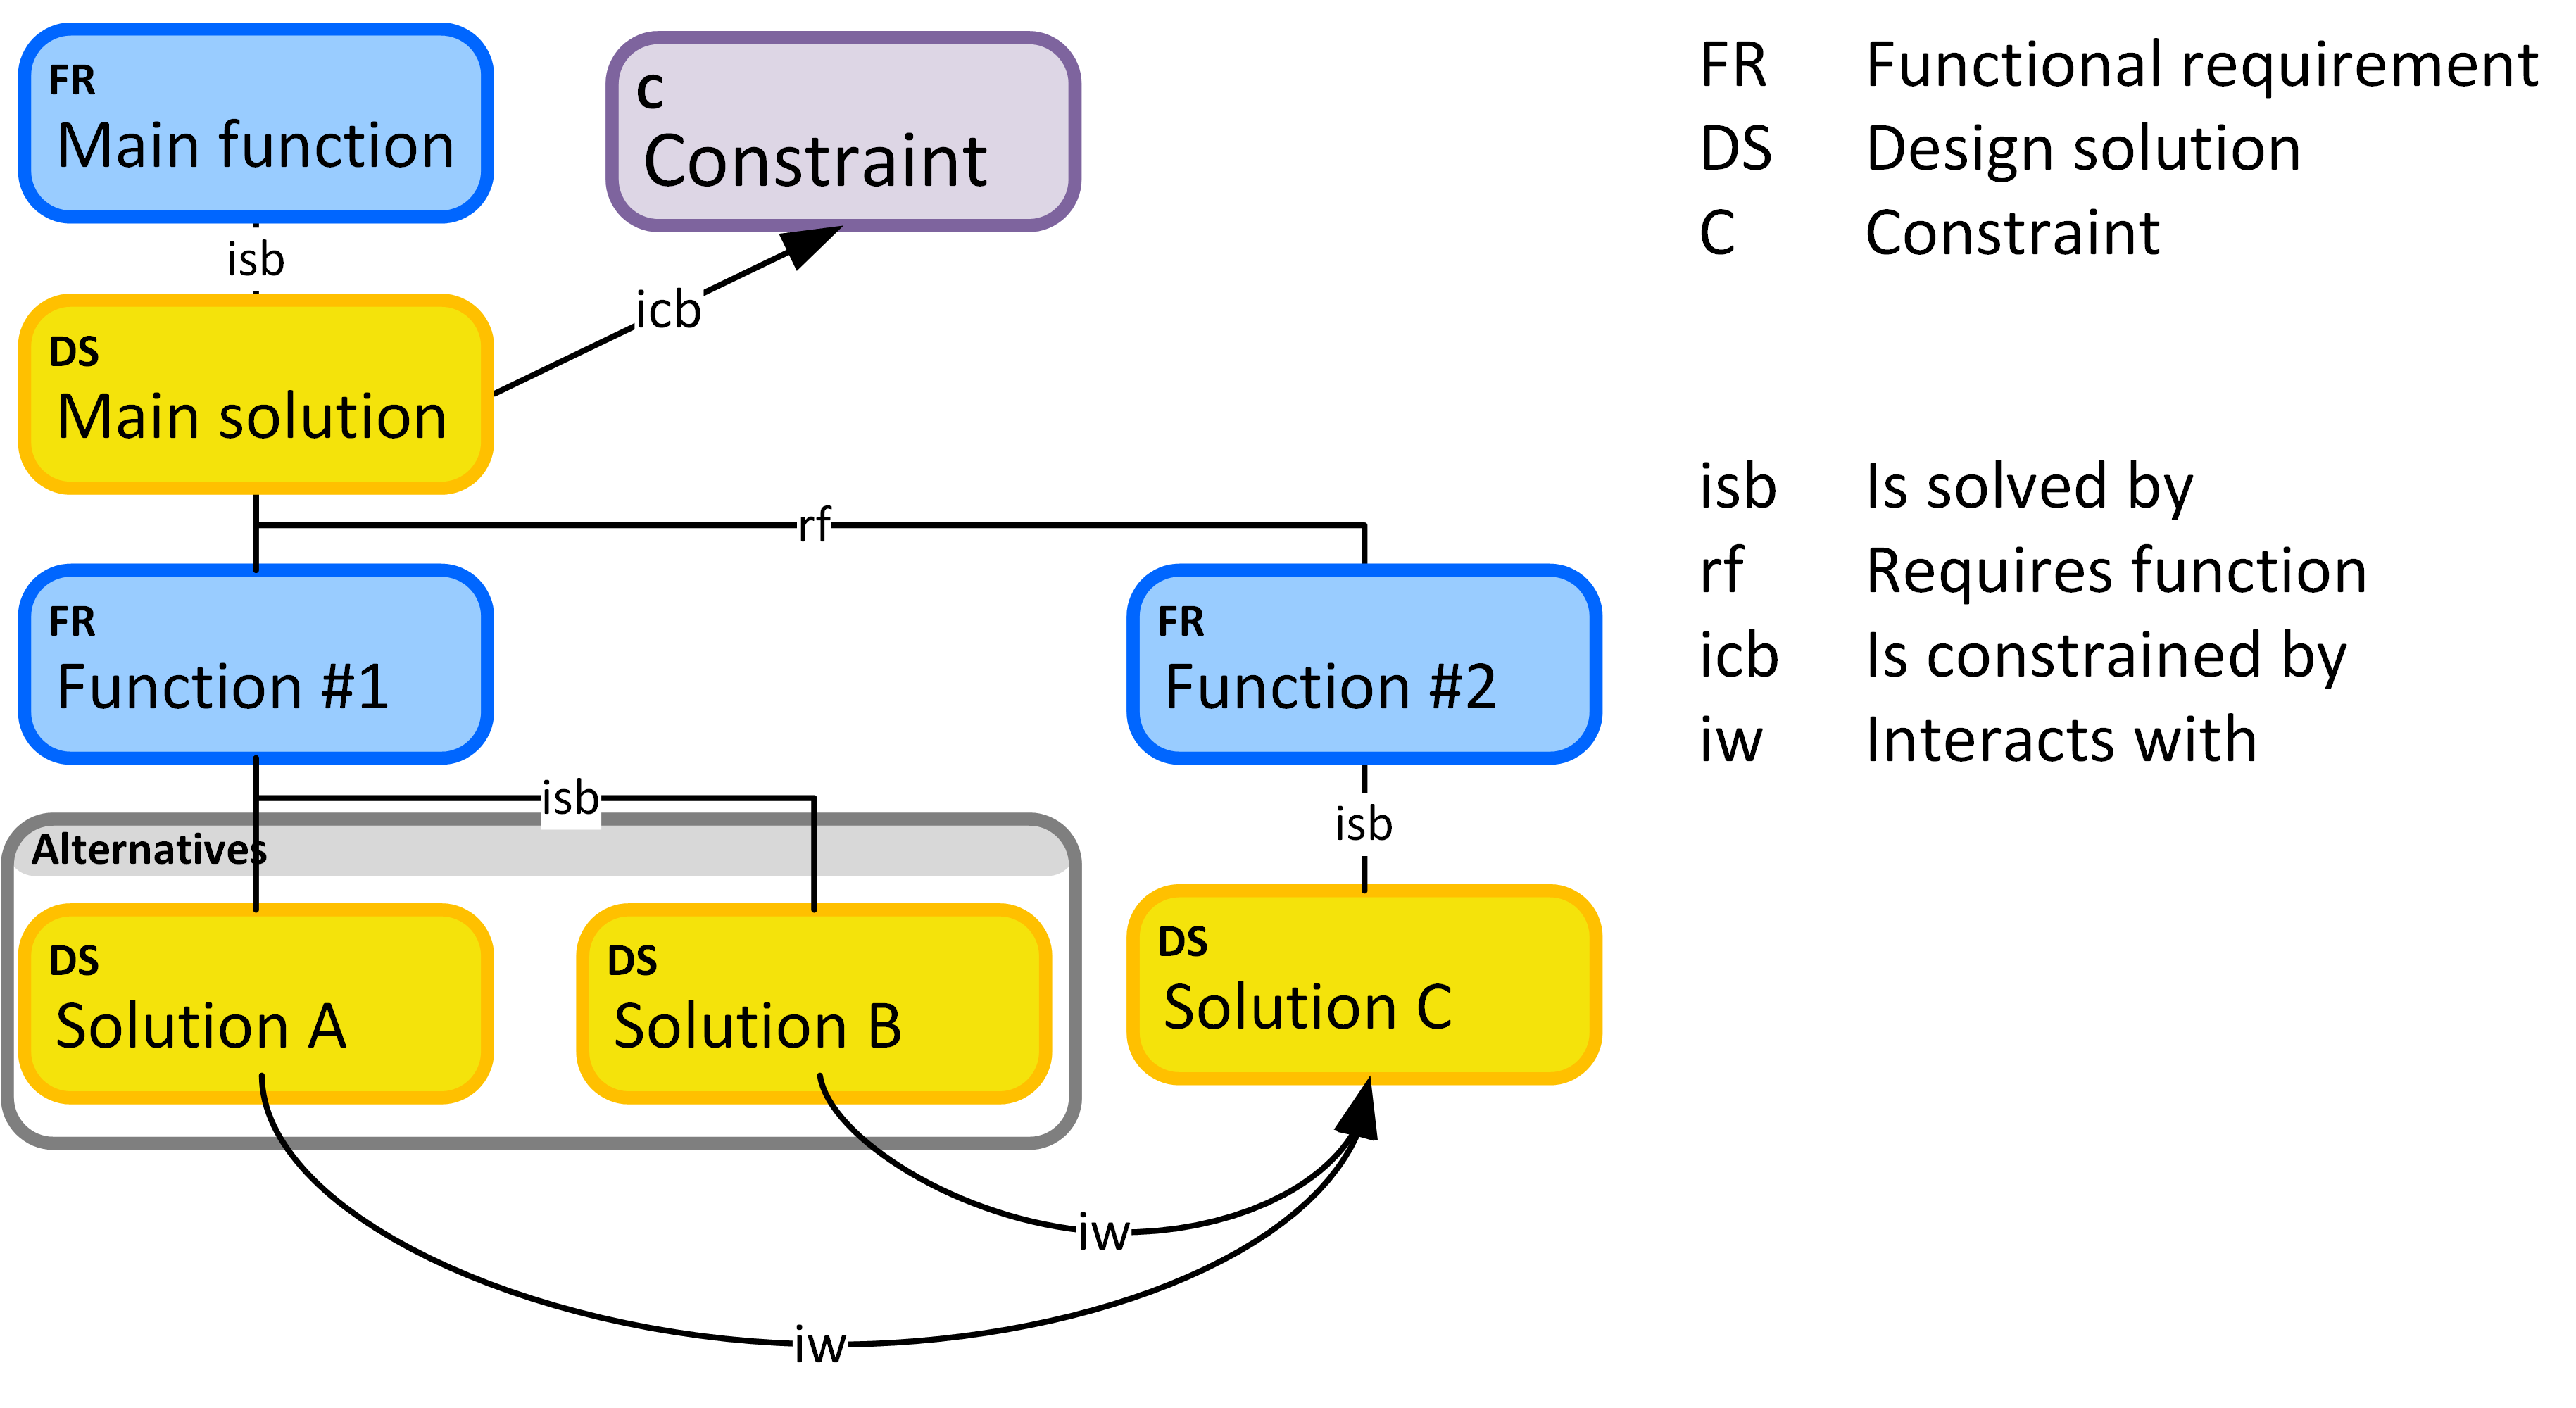
\includegraphics[width=.6\textwidth]{figures/efmExplanationBright.png}
    \caption{Enhanced Function-Means modelling elements after \cite{Schachinger2000}.}
    \label{fig:EFM}
\end{figure}

% instantiation
Since new \ac{DS} are captured for different functions on individual branches of the EF-M tree, they can be combined into a multitude of different concepts.
In the presented example in Figure \ref{fig:EFM}, only two concepts can be instantiated, one with each alternative \ac{DS}.
The \textit{instantiation algorithm} that has been implemented in \ac{FGE} also manages alternatives on arbitrary sub levels of the \ac{EF-M} tree.

% CAD / DA / UDF
To enable the generation of a CAD model of each design concept, a modularised \ac{DA} approach enables the assembly of individual CAD models based on their EF-M model.
The approach is presented in \cite{Muller2021FunctionVariants}.
Each \ac{DS} is coupled with \ac{UDF}, individually configurable CAD modules, which represent the geometry embodying the respective solution.
Since \ac{UDF} are as a functionality available in most commercial CAD systems, these geometry modules can be generated and edited by CAD engineers with minimal additional training.
Through the flexibility of \ac{UDF} and the possibility to parameterise them, this enables a fine granular control of the geometry via the \ac{EF-M} model.
The interfaces between the \ac{UDF} -- and therefor \ac{DS} -- are captured in the \ac{EF-M} model as \ac{iw} connections.
An assembly algorithm automatically generates the CAD models of all technically feasible concepts in the \ac{EF-M} model.

%\Jakob{presentation of the approach; EF-M model; CAD coupling; instantiation - more or less a short rundown from CADandA}

% aim of FGE: DSE, holistic, knowledge, CAD models for analysis

% base working principle: decomp, inno, embody
The \ac{FGE} approach is based on three main phases: functional decomposition of the legacy CAD model, an innovation stage in the functional domain and an embodiment step to realise CAD models for analysis.
Since the embodiment of all concepts has shown to be a key obstacle in investigating into multiple concepts, previous research \citep{Muller2020a} has yielded a modular CAD modelling approach that allows for the generation of CAD models of variant designs based on embodiment of only single \ac{DS}.


% The number of possible concepts, and therefore the portion of the explored design space\footnote{
% The number of concepts calculated by Equation \ref{eq:instantiation} covers the \textit{modular bandwidth} of the design space.
% \textit{Parametric bandwidth}, as described by \cite{Levandowski2013} however, is neglected in this study.},
% is presented here as a recursive function in Equation \ref{eq:instantiation}.

% % equation for all instances
% \begin{align}\label{eq:instantiation}
%     n_{concepts}(DS) &= \prod_{i=1}^{n_{fr}} altFR_{i} \\
%   \text{where recursively for all $altFR_i$:}& \\
%     % recursive equation for instances of subFR
%     altFR &= \sum_{j=1}^{n_{ds}} n_{concepts}(DS_i)\\
%     \text{subject to} & \\
%     altFR &\neq 0 
% \end{align}
% % variables in equation for instances
% \begin{align*}
%     \text{where} & \\
%     n_{concepts}(DS) &= \text{number of sub-concepts of a DS} \\
%     n_{fr} &= \text{number of FR of a specific DS} \\
%     n_{ds} &= \text{number of DS of a specific FR} \\
%     altFR &= \text{number of alternative solutions for a function} 
% \end{align*}    

Since each new \ac{DS} on any point in the function model leads to a factorial increase of concepts, an automatic generation of the CAD models is necessary to be able to analyse and evaluate all concepts.
% DA element
This is realised by the function-based modular geometry approach and assembly algorithm of \ac{FGE}.
Following this approach, presented and verified in \cite{Muller2021FunctionVariants}, the geometry not for each new concept has to be remodelled, but only for each new DS, which reduces the cost of introducing new product concepts based on a legacy design.
This modularisation, including a precise interface capture and management through the \ac{FGE} object model, allows for automated generation of the CAD models of all feasible concepts.



%%%%%%%%%%%%%%%%%%%%%%%%%%%%%%%%%%%%%%%%%%%%%%%%%%%%%%%%%%%%%%%%%%%%%%%%%%%%%%%%%%%%
%%%%%%%%%%%%%%%%%%%%%%%%%%%%%%%%%%%%%%%%%%%%%%%%%%%%%%%%%%%%%%%%%%%%%%%%%%%%%%%%%%%%
%%%%%%%%%%%%%%%%%%%%%%%%%%%%%%%%%%%%%%%%%%%%%%%%%%%%%%%%%%%%%%%%%%%%%%%%%%%%%%%%%%%%
\section{Materials and Methods}\label{sec:method}
% context @GKN
This study is conducted in collaboration with a Swedish aerospace manufacturer, and is centered around the design of a new part for turbofan engines, an Outlet Vane Guide (\ac{OGV}).
The part is located in the bypass of the turbofan engine, positioned just behind the fan, as shown in Figure \ref{fig:ogvInTurbine}.
The set of all \ac{OGV} has the main function to deswirl the airflow from the main rotor, thereby reducing aerodynamic losses.
Furthermore, the vane has a structural function in that it connects the shroud of the bypass to the \ac{FCB}, thereby creating a load path for the turbine mass to the pylon.
Furthermore, the part has to withstand axial loads from the engine thrust.

The development of \ac{OGV} is commonly subject to high weight reduction goals, which is met by the introduction of new manufacturing and material options.
The common manufacturing and material choice is a titanium core structure, partly hollow metallic \cite{Sjunnesson2019}.
Alternative options are composites or combined solutions.

% \begin{figure}[ht]
%     \centering
%     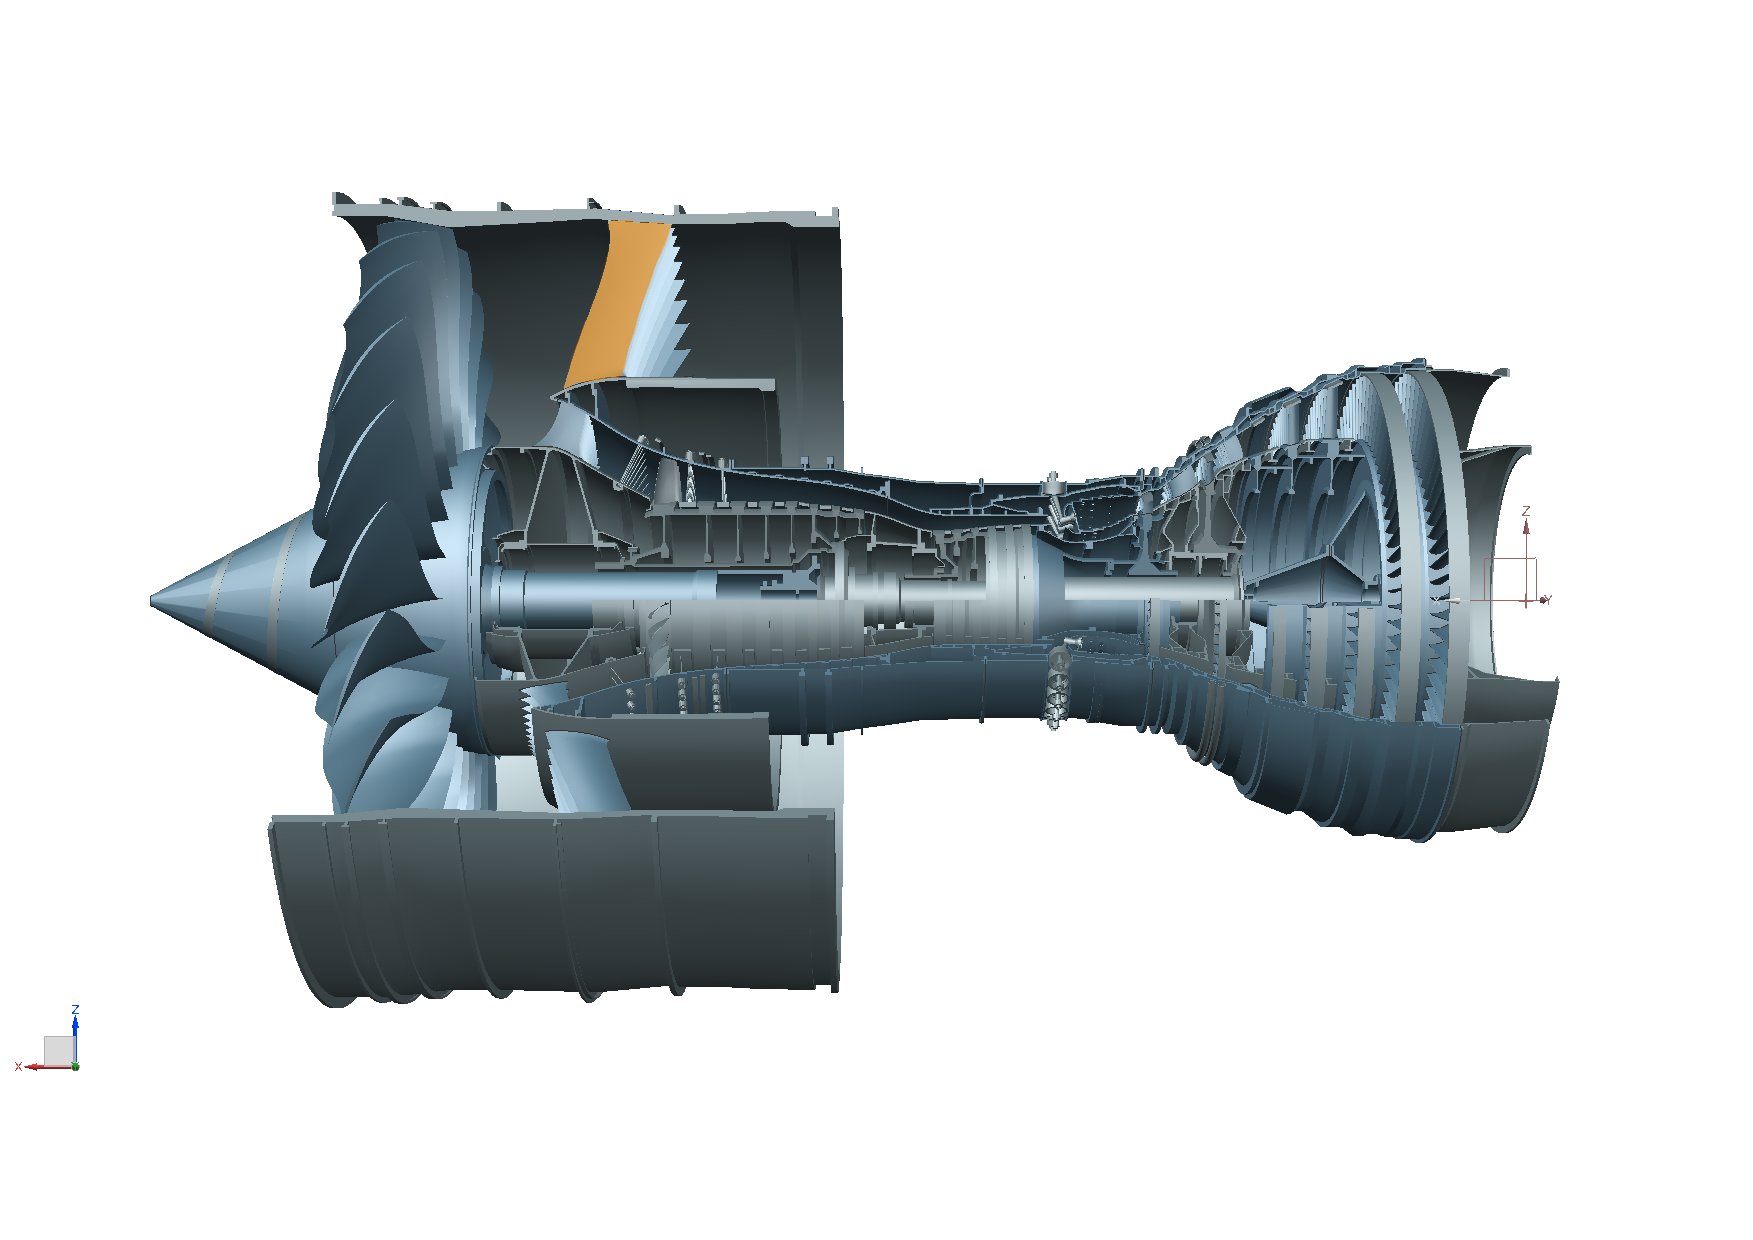
\includegraphics[width=0.9\textwidth]{figures/trent9000_OGV.png}
%     \caption{A Rolls Royce Trent 900 turbine rendered in CAD\protect\footnotemark, with one \ac{FF} \ac{OGV} highlighted in orange. \Jakob{add a render of an OGV as a figure b}}
%     \label{fig:my_label}
% \end{figure}

% figure of trent900, OGV
\begin{figure}[th!]
    \begin{center}
    \centering
        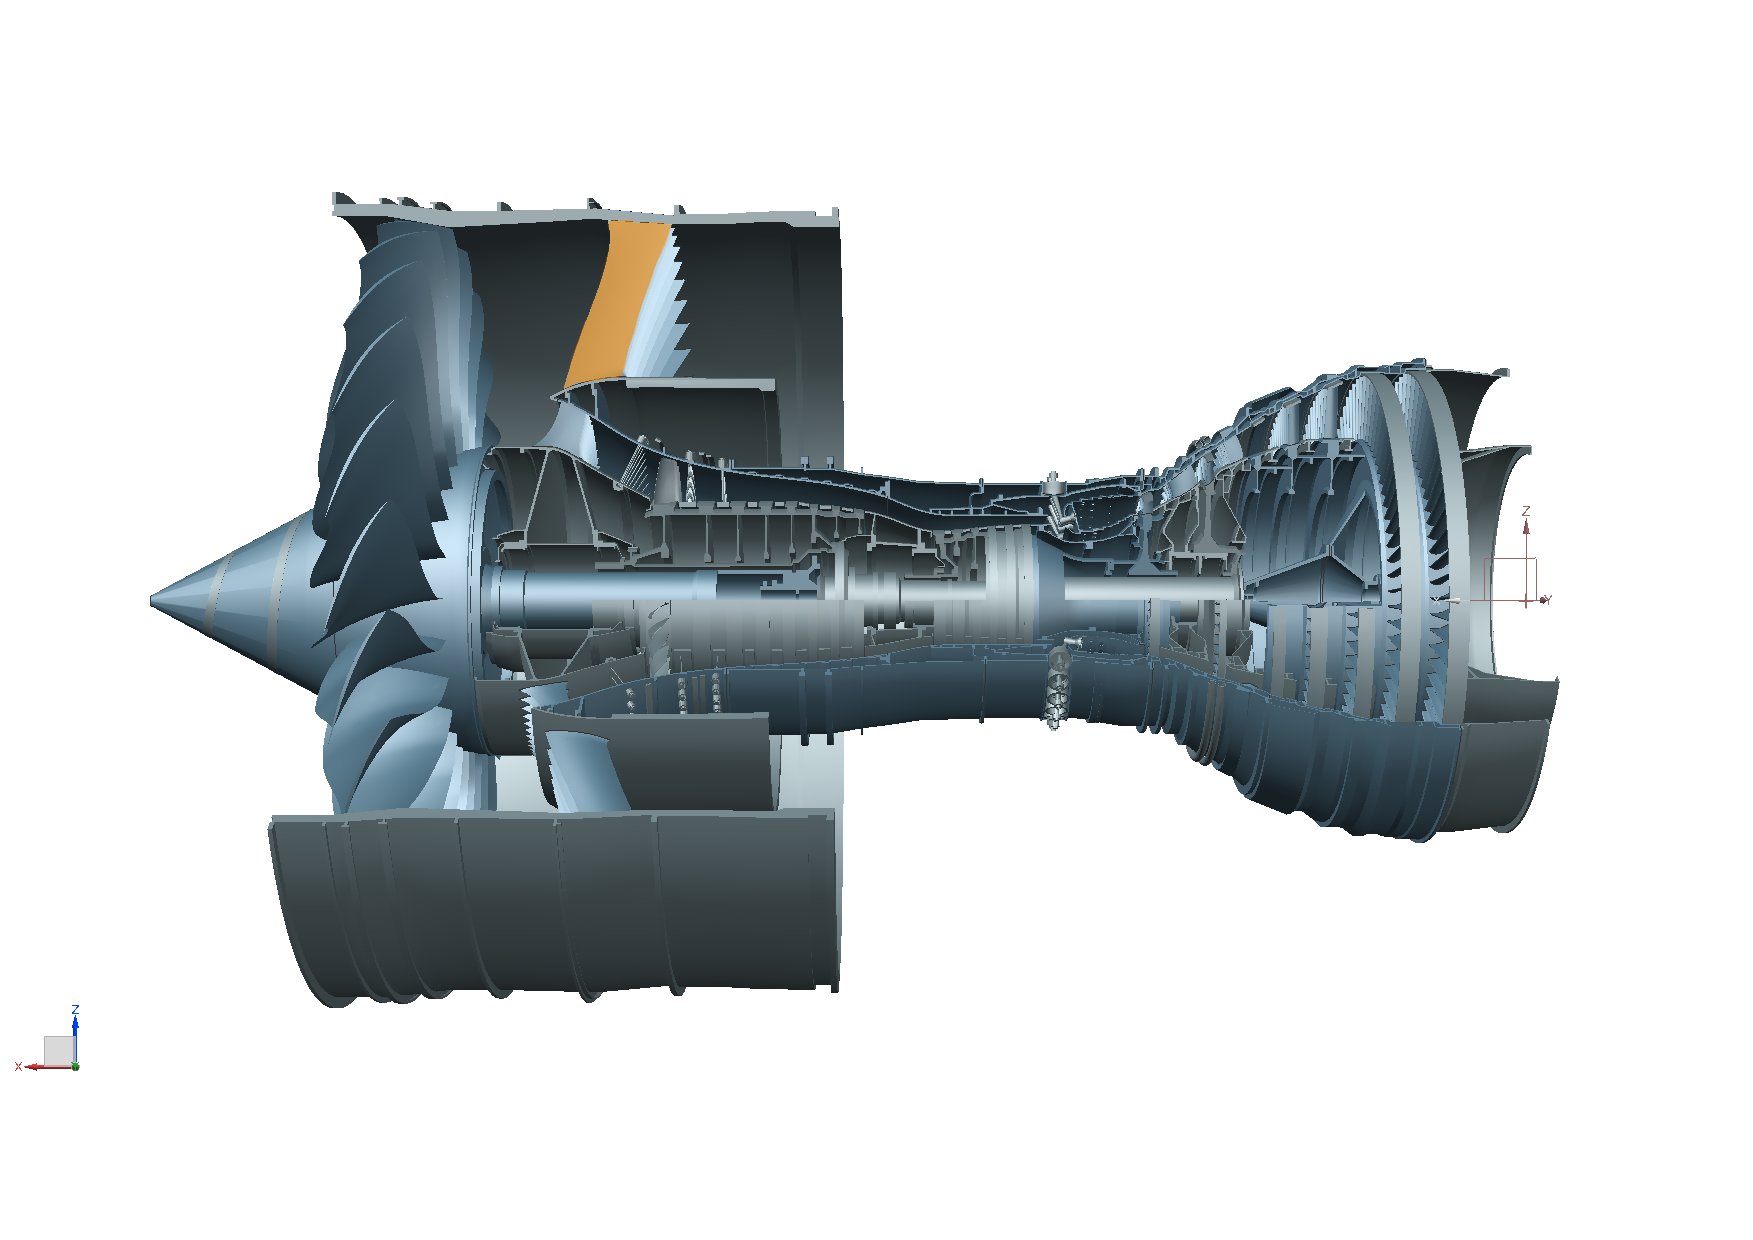
\includegraphics[width=\textwidth]{figures/trent9000_OGV.png}

        \caption{(A Rolls Royce Trent 900 turbine rendered in CAD\protect\footnotemark, with one OGV highlighted in orange.
        }
        \label{fig:turbine}
    \end{center}
\end{figure}

\footnotetext{CAD model by Chris Shakal on grabcad.com}
%\Jakob{present an illustration of the simple sample vane, geometry and EF-M}

An \ac{OGV} commonly consists of a vane structure, a predominantly aerodynamically defined structure, and two fittings which fasten the vane to a hub on the inside, and the outer fan case on the outside, as can be seen in \ref{fig:turbine}.
Both parts provide interfaces the \ac{OGV} assembly has to comply to.

In the company, the part is currently under redesign and development by a multidisciplinary team of more than ten engineers.
These engineers partake in the development in defined percentage of their work-time, between 10\% and 70\%. It is important to mention that the company is since the late 90s heavily investing on the development of KBE techniques for design space exploration, based on state-of-the art CAD parametric modelling approaches. This means that the engineers possess a benchmark system for comparison with the FGE. This allowed to highlight potential benefits and implementation issues.    

% action research framework
The project is performed in an action research approach, where the researchers accompany the development process investigating into new opportunities for a fan frame \ac{OGV} \citep{Yin2006}.
The researchers participate in certain regular team meetings of the development team, and have the ability to observe the engineers during their work.
Notes from these meetings and observations are part of the data supporting the presented results.

\subsection{Study setup}
Beyond the observation throughout the regular development approach, a set of studies has been setup to investigate the perception of the presented method.
The majority of data collection was performed in two workshops.

% initial interviews???

% workshop 1 and decomposition
In a first workshop together with the \ac{OGV} development team (eight participants), a functional decomposition of the part was performed and captured.
Hence, this workshop is referred to as the "decomposition workshop".
The actual workshop was predated with a one hour long test-workshop in one of the regular team meetings to evaluate the motivation of the practitioners and the requirements for the actual workshop.
The results of this "test-workshop" are included in the results of the decomposition workshop.
The decomposition was performed using large-scale print-outs of drawings an \ac{OGV} which were annotated in a group exercise.
The annotated drawings were collected, digitised and used for the creation of function-geometry model in \ac{FGE} for the legacy design.
%After the decomposition activity, the practitioners were asked to fill out a questionnaire about their perception of the workshop.
%The workshop was concluded with an open feedback round.

%workshop 2
A second workshop (eight participants) covered the innovation stage of the \ac{FGE} approach. 
The workshop was done with the same development team, using the same product.%, although due to scheduling challenges the participant groups in workshop one and two were not exactly identical, but each engaged 80\% of members the development team.

% prototype tool
For the second, online\footnote{The workshop was performed online due to the social distancing regulations caused by the COVID-19 pandemic.}, workshop a prototype tool of the \ac{FGE} approach was created.
The tool works server-based with a web interfaces, allowing users with different skill levels and operating systems to connect to the same database.
The tool incorporates a fully functional implementation of an \ac{EF-M} modeller with additional functionality to capture geometric information for each \ac{DS}.
As such, it is able to capture alternative design solutions and instantiate them into different concepts.
Furthermore did the tool include a geometrical modelling aspect to automatically generate \ac{CAD} models of each concept, based on previous geometrical modularisation in Siemens NX.
The structure and mechanics of the tool have been illustrated by \cite{Muller2020a}.

% data capture and analysis
After each workshop, the practitioners were asked for their experiences through questionnaires and open feedback.
The results of the first workshop were recorded through adhesive notes and remarks on the drawings, as well as protocol notes.
The results of the online workshop were captured through audio and video recording and through a change protocol in the database of the \ac{FGE} tool.

%The findings from the workshop were verified through semi-structured in-depth interviews with selected participants of the workshop. \Jakob{these are still outstanding - hopefully after summer!} 

Since the product being in development at the case company, it underlies certain \ac{IP} and export restrictions. 
Therefore, in this publication, a simplified model is used for presentation purposes in order to protect the case company's and their customers' \ac{IP}.
However, the simplified \ac{OGV} model has been verified with the practitioners in order to be able to convey the main functions and solutions of a generic \ac{OGV}.



%%%%%%%%%%%%%%%%%%%%%%%%%%%%%%%%%%%%%%%%%%%%%%%%%%%%%%%%%%%%%%%%%%%%%%%%%%%%%%%%%%%%
%%%%%%%%%%%%%%%%%%%%%%%%%%%%%%%%%%%%%%%%%%%%%%%%%%%%%%%%%%%%%%%%%%%%%%%%%%%%%%%%%%%%
%%%%%%%%%%%%%%%%%%%%%%%%%%%%%%%%%%%%%%%%%%%%%%%%%%%%%%%%%%%%%%%%%%%%%%%%%%%%%%%%%%%%
\section{Results}\label{sec:results}

% interface for study, simple vane sample
To facilitate the interaction with the industrial practitioners, the \ac{FGE} approach has been developed into a proof-of-concept tool. The tool has been developed as a server-based application with a web-interface. 
The web-interface is presented in Figure \ref{fig:omfgDSEinterface} and shows a simplified EF-M tree of an \ac{OGV}. 
Using this simplified \ac{OGV} model, the practitioners were introduced to the \ac{EF-M} modelling using the \ac{FGE} tool, and given a presentation of the \ac{DA} component of \ac{FGE}.

The next sections describe how the design space exploration of the OGV has been conducted with the industrial practitioners with the support of FGE. 
Also, it will describe the practitioners' feedback and reflections after the use of the method.
%The respective CAD models of the demo-geometry are shown in \ref{fig:}.

\begin{figure}[ht]
    \centering
    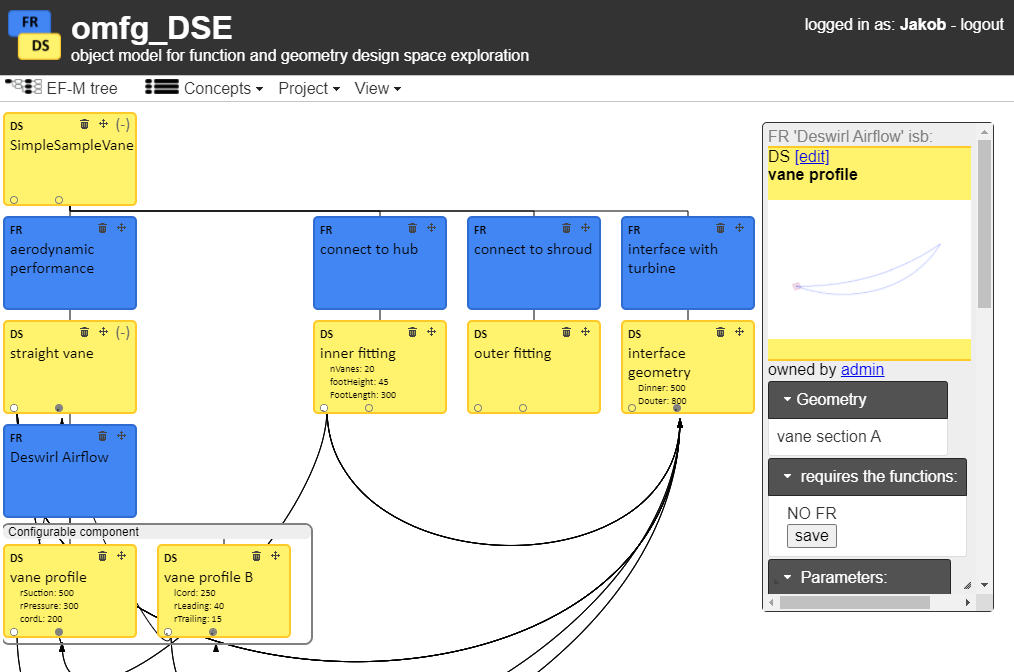
\includegraphics[width=0.8\textwidth]{figures/omfgDSEinterface.png}
    \caption{Web-based interface of the FGE tool "omfgDSE" (object model for function and geometry based design space exploration) , showing a simplified EF-M model of an OGV.
    The right-hand box illustrates the details of a DS, such as associated geometry and parameters.}
    \label{fig:omfgDSEinterface}
\end{figure}

%%%%%%%%%%%%%%%%%%%%%%%%%%%%%%%%%%%%%%%%%%%%%%%%%%%%%%%%%%%%%
\subsection{Design space exploration using FGE}
The \ac{DSE} approach is separated into three phases \textit{decomposition}, \textit{Innovation} and \textit{embodiment}, following \cite{Muller2019Aiedam}.
The presented workshop focuses on the interactions with practitioners in the phases decomposition and embodiment.

% Decomposition
%\subsubsection{First workshop - Decomposition}

In the\textit{ first workshop (decomposition)}, the legacy design of the \ac{OGV} was decomposed into a \ac{EF-M} model.
The model contained three main functions, and 18 different design solutions on the concrete (lowest) level.
Since the model was created through decomposition, all \ac{DS} were directly linked to one or several geometry elements.
A modularised CAD model was created based on the original geometry, but modularised according to the decomposition.
% introduce here the new figure

% \begin{figure}[ht]
%     \centering
%     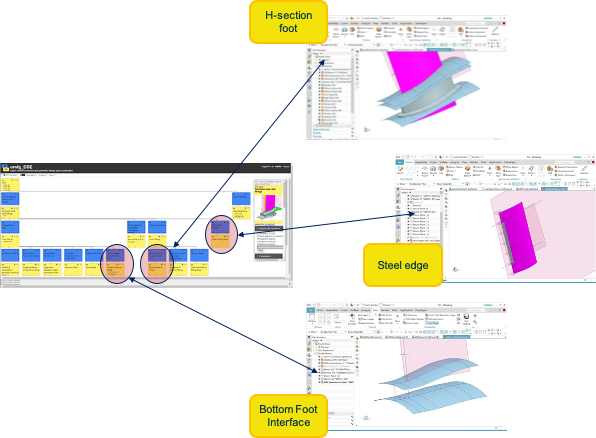
\includegraphics[width=\textwidth]{Picture 2.png}
%     \caption{Connection between the modularized CAD model of the legacy design, directly linked to the DSs in the EF-M model.}
%     \label{modularizedCAD}
% \end{figure}

Figure \ref{fig:decompositionExample} shows this connection for four distinct DSs.
For example, the leading edge of the decomposed \ac{OGV} is covered by a steel edge.
This steel edge, as a geometrical element, has been associated with the function "Withstand impacts" through the solution "Steel edge".
The respective geometry, the part of the steel edge and the cutout in the vane shape to place it, are captured in a UDF which are then associated with the DS.

%Other examples of geometry elements connected to DSs are "H-section foot" and "Bottom Foot Interface". 
This decomposition served as input for the following workshop, focused on innovation. 

% introduce here a connecting sentence witht he next 
% new solutions
%\subsubsection{Second workshop - Innovation}

In the \textit{second workshop (innovation)} used the prototype tool to capture the novel design solutions.
In this process, the product model was extended by five new sub-functions that had been omitted in the previous workshop.
n this workshop, innovation was made first at the functional level - with the introduction of five new sub-functions for the OGV. For example,  sub-functions related to acoustic performances were added to the model. 
In the workshop, the practitioners found ten novel alternative  design solutions over the legacy design.
Their nature ranged from material alternatives over different interface approaches to variations in shape and dimensions of the existing solutions.
The entire EF-M tree, with all novel FR and DS highlighted with red borders, is shown in Figure \ref{fig:fullEFM}.
%Exemplary for the different new solution, one set of alternative DS is presented here in both the functional and geometrical domain, as well as the respective elements of the \ac{OMFG} linking those two domains.


\begin{figure}[ht]
    \centering
    
\includegraphics[width=\textwidth]{figures/fullEFM.png}
    \caption{Complete EF-M model after the innovation workshop.
    All new DS and FR are highlighted with a red border.
    Readability has been dismissed on purpose to protect company IP.}
    \label{fig:fullEFM}
\end{figure}

% new solutions example
The majority of the novel solutions shows a conceptual difference from the legacy design.
As an example, the \ac{FR} "Join vane to fitting" is in the legacy design solved by the \ac{DS} "Adhesive connection", meaning that the vane is glued to the fitting using resin.
The two alternative \ac{DS}, as results from the workshop, were "Bolted joint" and "Fully integrated solution".

%subsubsection{Embodiment}

% maybe we should not bring this:
The \textit{embodiment} phase of the \ac{FGE} approach has not been performed in its entirety, since the \ac{DA} section of the proof-of-concept tool has not sufficiently matured to handle the complex geometries of the solutions devised in the innovation workshop. For a verification of the proof-of-concept tool on another turbine structure, see \citep{Muller2021FunctionVariants}.

% alternative:
Based on the different alternative solutions and functions captured in the innovation workshop, 52 different concepts were instantiated.
The respective solutions were embodied and combined.

Figure \ref{fig:altOGV} shows an exemplary embodiment of three concepts with alternative DS for the FR "Join vane to fitting" shown in Figure \ref{fig:efmAltFoot}.
While otherwise using the same configuration, each of the geometries is adapted to accommodate the respective geometric changes in the concept.

\begin{figure}[ht]
    \centering
    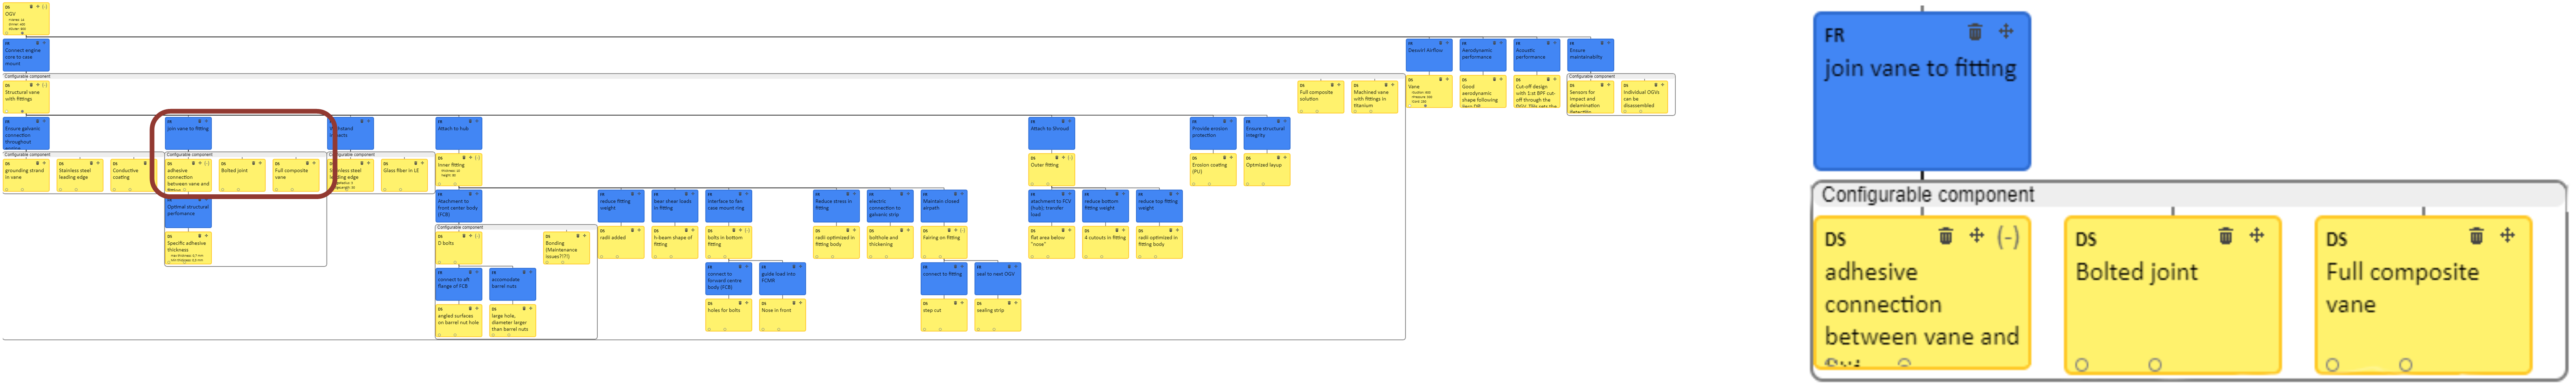
\includegraphics[width=\textwidth]{figures/efmHighlightFoot.png}
    \caption{Detail of EF-M tree after innovation workshop: alternative solutions for DS "Join vane to fitting".}
    \label{fig:efmAltFoot}
\end{figure}


\begin{figure}[th!]
    \begin{center}
    \centering
        \begin{subfigure}[b]{0.3\textwidth}
            \centering
            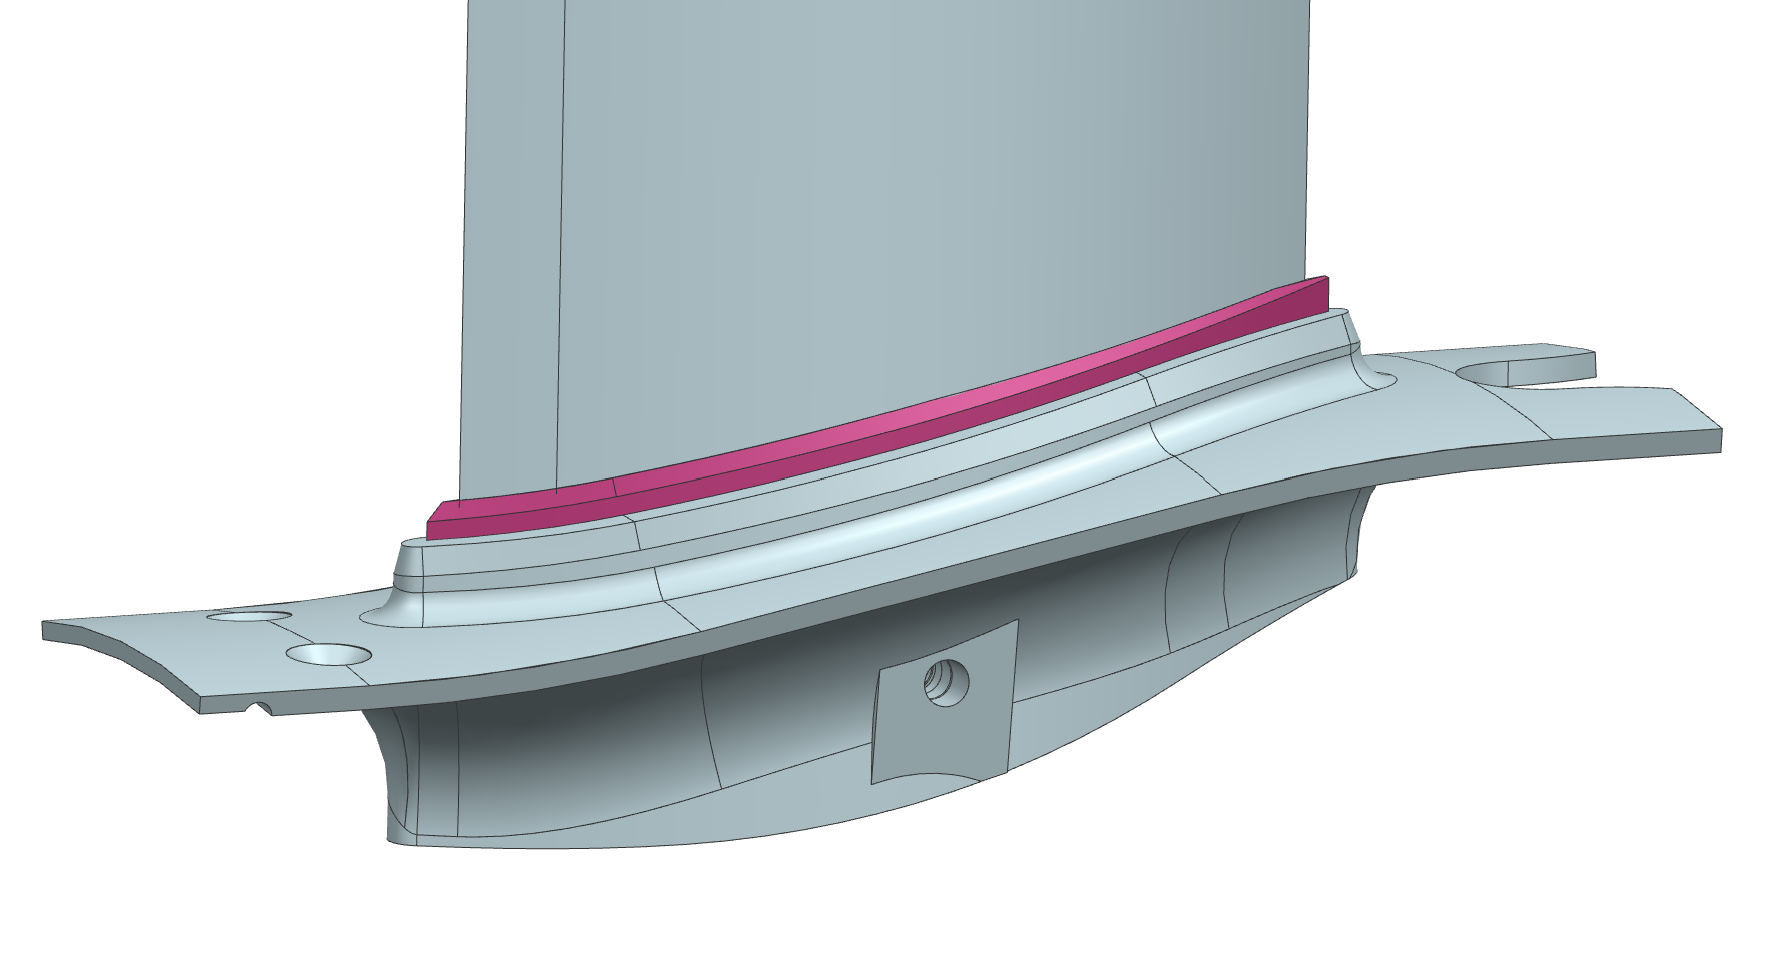
\includegraphics[width=\textwidth]{figures/footGluedCad.png}
            \caption{}
            \label{fig:turbofan}
        \end{subfigure}
        \hfill
        \begin{subfigure}[b]{0.3\textwidth}
            \centering
            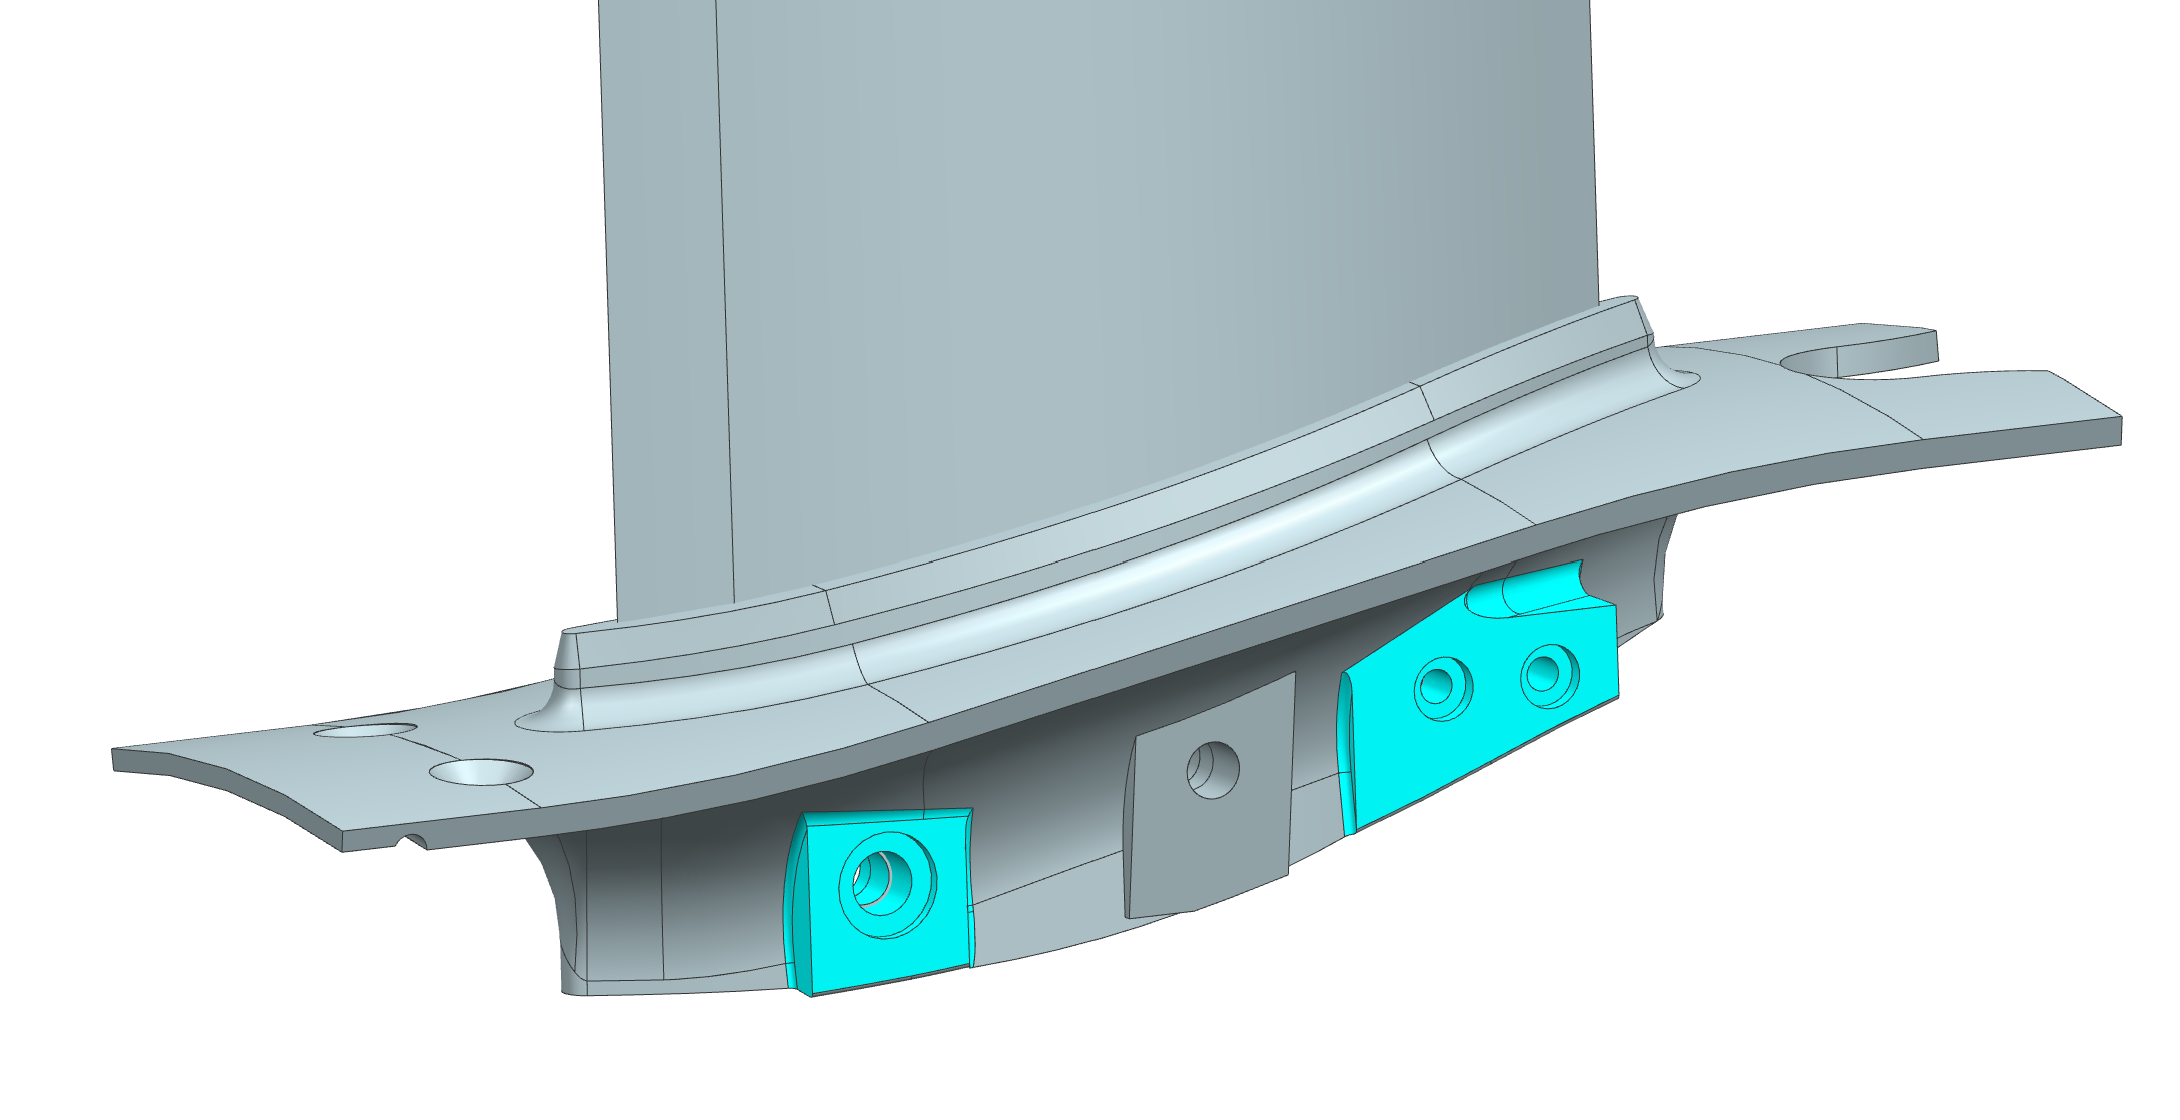
\includegraphics[width=\textwidth]{figures/footBoltedCad.png}
            \caption{}
            \label{fig:ogvRender}
        \end{subfigure}
        \hfill
        \begin{subfigure}[b]{0.3\textwidth}
            \centering
            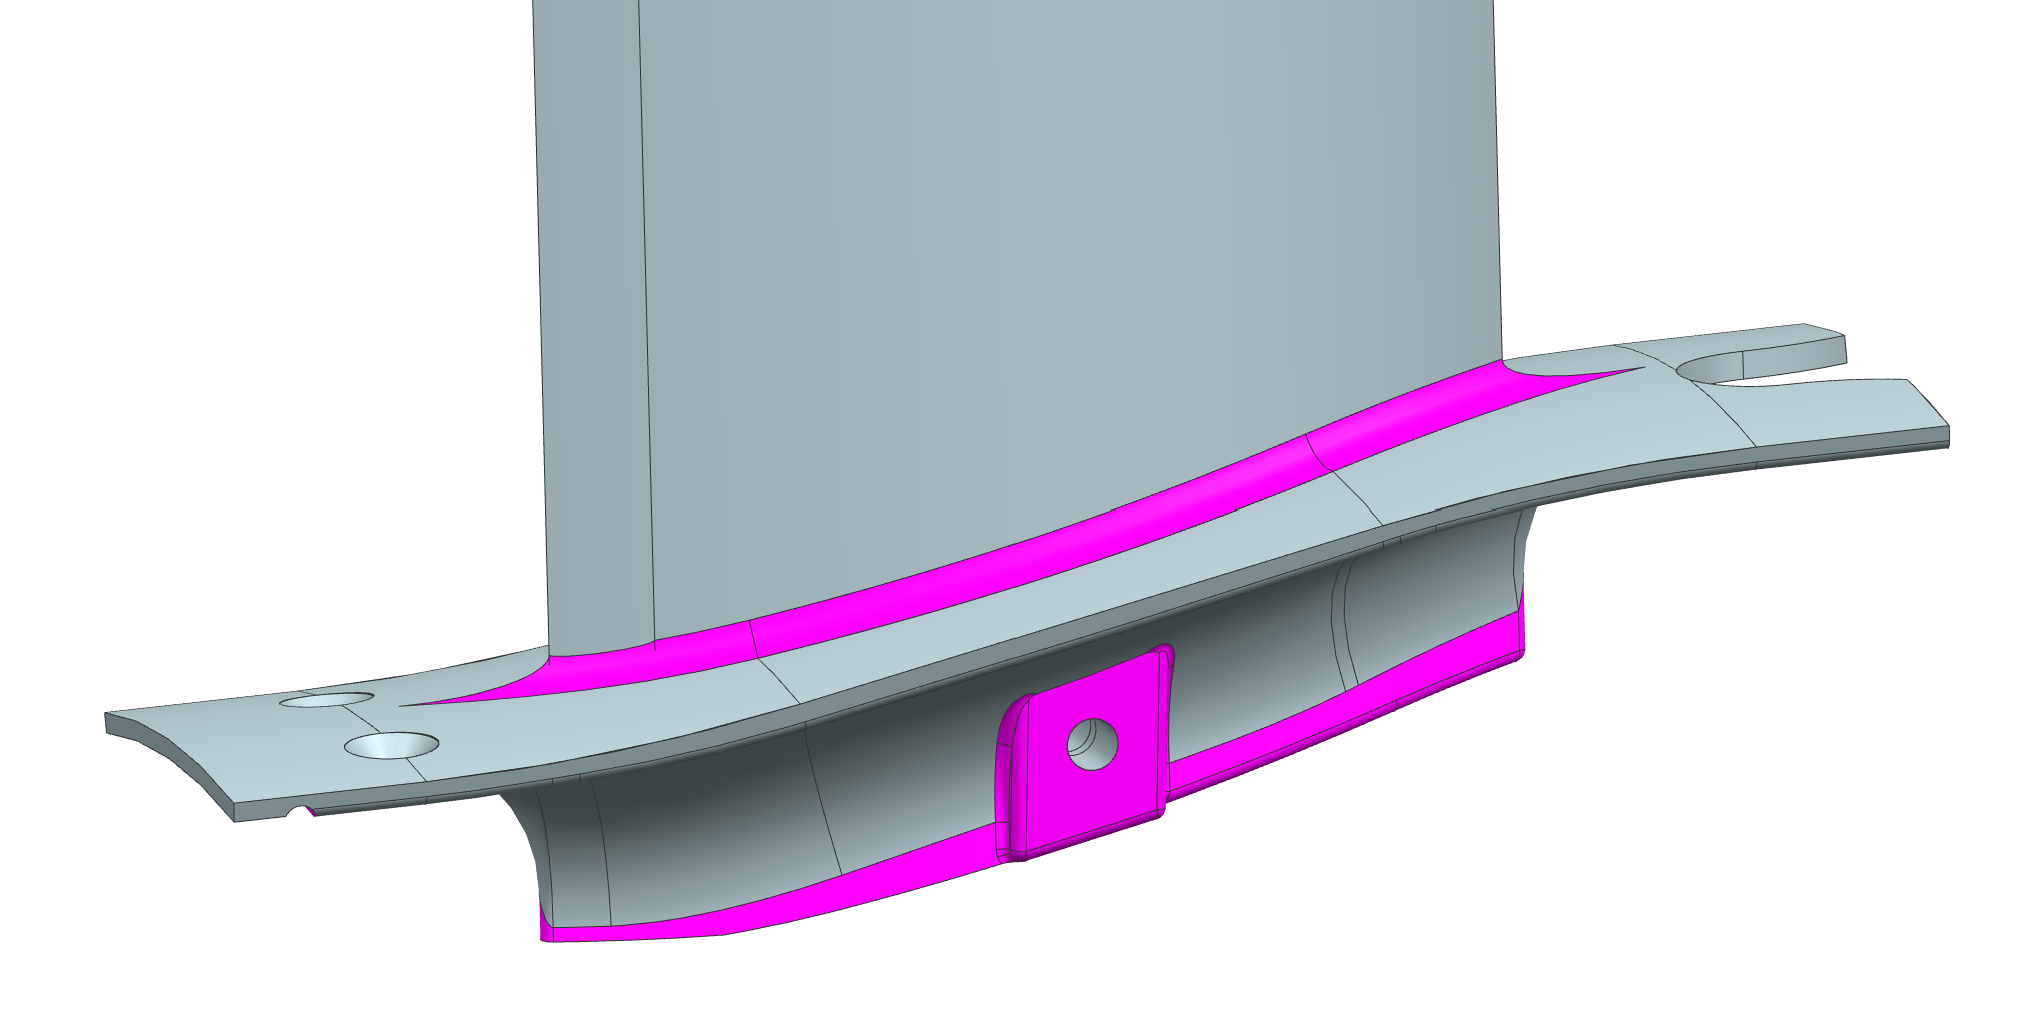
\includegraphics[width=\textwidth]{figures/footOnePiceCad.png}
            \caption{}
            \label{fig:ogvRender}
        \end{subfigure}
        \caption{Embodiment of three concepts, differentiating in the solutions for the FR "Join vane to fitting", from left: (a) "Adhesive connection", (b) "Bolted joint" and (c) "Fully integrated solution".
        Respective alternative geometric elements relating to the respective UDF are highlighted in colour.}
        \label{fig:altOGV}
    \end{center}
\end{figure}

The instantiation and assembly algorithms embedded in the FGE model allows for automated generation of the CAD models of all feasible concepts - through combinatorial assembly.  

The following section reports on the practitioners' feedback and reflections after the application of the method on their industrial use case. 

% Each of the solutions was modelled as a \ac{UDF} in Siemens NX, and the resulting UDF was coupled to the EF-M model through the \ac{OMFG}.
% %The resulting \textit{UDF} and \textit{interface} objects in the \ac{OMFG}, as well as the geometry, are illustrated in Figure \ref{fig:altSolutionOmfg}.

% % instantiated 
 % geometry
% The technical feasibility of automated geometry generation was assessed based on experiences with the \ac{FGE} modelling approach in a previous study with a similar turbofan engine part, see \cite{Muller2020a}.
% This qualitative assessment of the new concepts showed that approximately $35$ of the 52 theoretically possible concepts could be realised as CAD models, using the modular \ac{DA} approach of \ac{FGE}.
% \Jakob{
% In the workshop, 10 relevant new DS were introduced (compared to legacy design)

% 2 new functions were introduced

% total of 52 new concepts

% how many of these geometrifiable?

% }

%%%%%%%%%%%%%%%%%%%%%%%%%%%%%%%%%%%%%%%%%%%%%%%%%%%%%%%%%%%%%
\subsection{Reflections form industrial practitioners regarding the application of the method} \label{sec:feedback}

The general feedback from the industrial practitioners has been positive, with practitioners stating that the approach fit well into the development project -- albeit maybe too late -- and they would like to do similar workshops again on other products.
The following sections will go through the main mechanisms that have been highlighted by the industrial practitioners, in particular the ability of the approach to:

\begin{enumerate}
	\item Provide a clear and explicit illustration of the design rationale of the product. 
	\item Capture, integrate and model novel solutions.
	\item Provide a clear connection between the abstract functional and the concrete geometrical domain, which has the potential to foster innovation.
\end{enumerate}

\subsubsection{Ability to provide a clear and explicit illustration of the design rationale of the product }

\begin{center}
    “I learned a lot of things about the OGV just by reading the graph” 
\end{center}
\begin{flushright}
    -aerodynamics analysis engineer
\end{flushright}


This quote is representative of a common problem during the design of aerospace products. As components are designed and conceptualised over long times, and by a different people, it is difficult to retain the design rationale of a product (for example why the product looks the way it does). This problem has been identified in other sectors as well \citep{Bracewell2009}. 
For practitioners, the FGE approach supported the ability to clearly visualise the rationale in both the geometrical domain, visualising "what is", and the functional domain, "why it is".

It appeared to be most important to some practitioners that they improved their knowledge about the product and participated in a forum that permitted exchange about the product's functions and solutions.
The questionnaire accompanying the workshop revealed that no team member had full confidence about the \ac{OGV}, but the confidence in the team's knowledge was higher (2.9 out of 5 for individuals vs 3.7 out of 5 for the team).

\begin{figure}[ht]
    \centering
    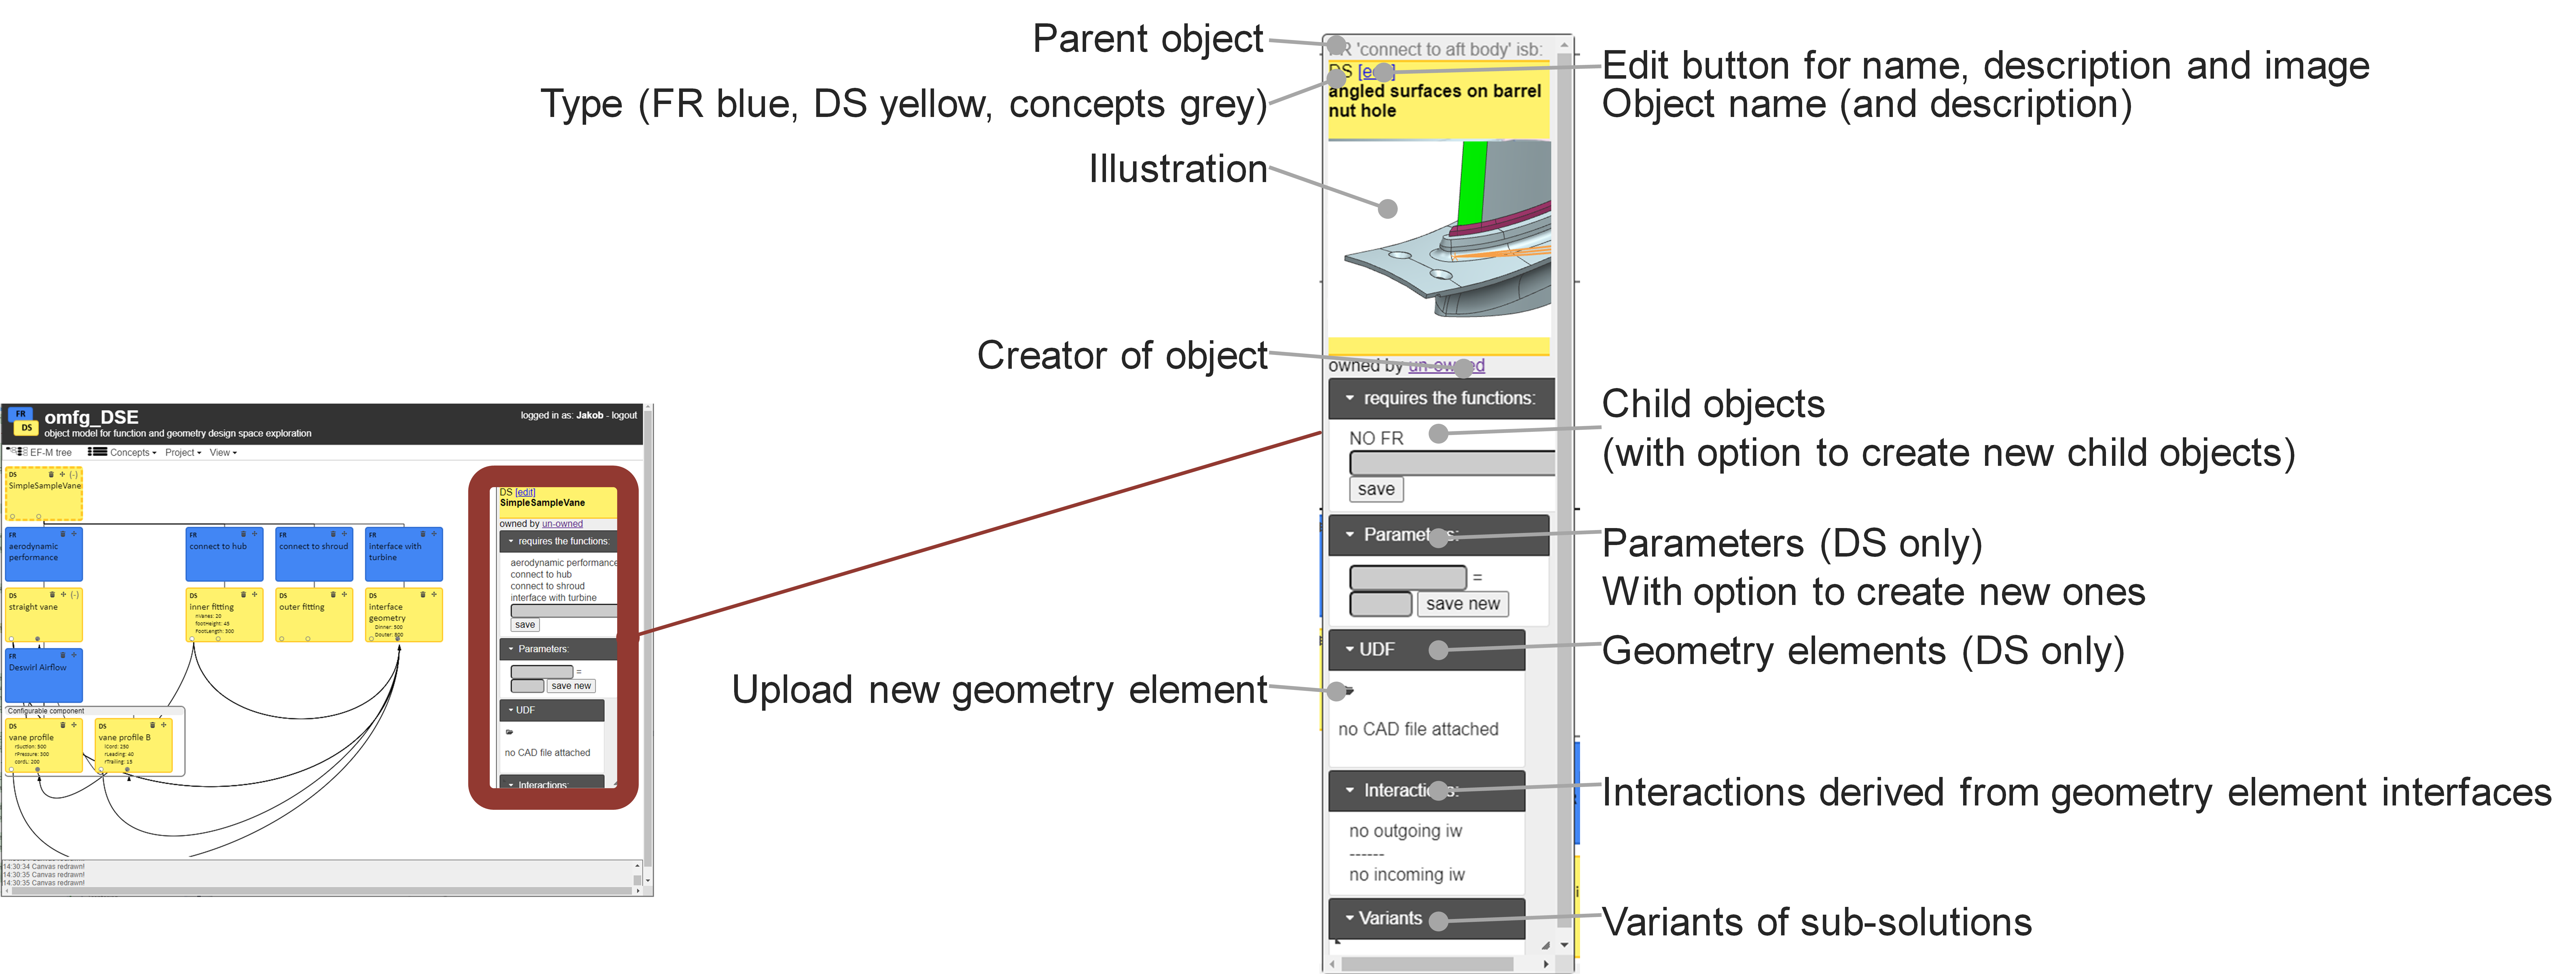
\includegraphics[width=\textwidth]{figures/validationDetails.png}
    \caption{Excerpt of the FGE interface that shows the design rationale of a geometry element. The parent FR is associated to the corresponding DS and geometry element}
    \label{fig:interface}
\end{figure}

As an example for how \ac{FGE} enables the acces to \ac{DR} is the interface of the tool used in the study, which collects all information of a solution in a single place.
Figure \ref{fig:interface} shows on the right hand side how the geometry, parameterisation and other information about a solution is collected in a single window pane.
The top of the pane shows which function is solved, and the highlighting of the solution shows its position in the product architecture.

Furthermore, the approach can illustrate the geometrical interfaces between solutions through \ac{iw} connectors in the \ac{EF-M} model.
This are seen as black arcs in the interface of Figure \ref{fig:interface}, left hand side, as well as Figure \ref{fig:omfgDSEinterface}.

Proofing this, most practitioners stated a higher knowledge of the product after the workshop than before.



%please comment the figure.
%redid the figure to hide the IP information and show iw connectors
% have to enlarge it though for readbility -.- but that takes too much time now
%also think i embedded it in the text ok?

%%%%%%%%%%%%%%%%%%%%%%%%%%%%%%%%%%%%%%%%%%%%%%%%%%
%%%%%%%%%%%%%%%%%%%%%%%%%%%%%%%%%%%%%%%%%%%%%%%%%%
\subsubsection{Ability to capture, integrate and model novel solutions. }

\begin{center}
    “Parametric solutions exist, where dimensions can be changed, limited to parameters that we change, dimensions or angles or that – but we cannot iterate over different design solutions, where it’s bigger changes” 
\end{center}
\begin{flushright}
    -- development team leader
\end{flushright}

\begin{center}
    “Right now our system for DSE is limited to changing parameters (dimensions, angles…) and does not iterate over different Design solutions” 
\end{center}
\begin{flushright}
    -- analysis/meshing specialist
\end{flushright}

\begin{center}
    “There are still gaps within early concept phase – this is one possibility to generate, and evaluate, lots of concepts, get trend curves and so on” 
\end{center}
\begin{flushright}
    -- design engineer
\end{flushright}
These three quotes represent instances of the practitioners' reflections over the in-house \ac{KBE} system for DSE adopted by the company, and built around state of the art KBE approaches.
while recognising the power of these techniques, they recognise that while the exploration of dimensional variations is well supported, the exploration of concepts which differ from the legacy design in \textit{topology} is limited.

According to the practitioners, FGE has the potential to deliver this through the modularisation of the geometry, and the connection to the \ac{DR} of the product.


% more solutions
It was perceived by the participants of the workshop that the use of the \ac{FGE} approach supports the introduction of new solutions ($4$ on a scale of $1$ "no support for new solutions" to $5$ "totally supports").
% novel solutions
It was furthermore stated that a part of the identified \ac{DS} would probably not have been found -- or considered -- in a regular modelling approach, with a majority ($71\%$) stating "maybe some, but not all".
The other participants stated either "none of them" or "most of them" without \ac{FGE}.

% more functions 
Beyond only exploring new solutions for existing functions, \ac{FGE} also enables the capture of newly identified functions or sub-functions.
Practitioners feedback supports this, although the ability to integrate new solutions is perceived to be better than that of new functions.

To summarise this, the practitioners perceive FGE as a viable method to capture novel solutions and functions.
It has been interpreted that FGE does so better than the parametric DSE approach in use at the company.



%%%%%%%%%%%%%%%%%%%%%%%%%%%%%%%%%%%%%%%%%%%%%%%%%%
%%%%%%%%%%%%%%%%%%%%%%%%%%%%%%%%%%%%%%%%%%%%%%%%%%

\subsubsection{Ability provide a clear connection between the abstract functional and the concrete geometrical domain }


\begin{center}
    “what we are looking for is how to get an efficient concept generation phase before we go into our parametric system [\textit{author's note: the in-house systems for DSE}]  –- so that we get an overview over potential concepts ” 
\end{center}
\begin{flushright}
    -- development team leader
\end{flushright}



% Especially in aerospace components, due to strict constraints on weight and high requirements on performance, the products turn out to be highly integrated \citep{Raja2019}.
% As a result, only few team members have an overview over the \ac{DR} of the product. 
% This has also been observed in the workshops.
% Only one team member was relatively confident in their knowledge about the part, whereas the others had only segmented knowledge and judged their knowledge with an average of 2.7 out of five.

%identified areas for improvement through decomposition as well as identified "do not touch"
Almost all participants stated that through the decomposition workshop, "do not touch" areas as well as areas for improvement on the product could be identified.
This provides a clearer representation of the design space for the engineers: 
through the mapping of geometry to function, the "do not touch" areas become tangible in \textit{why} they shouldn't be altered, and furthermore what impact this has on the rest of the product architecture, with a participant representatively stating it was interesting to see "how it is connected"
This is a major strength of the direct coupling of the function to the geometry model:
Other modelling approaches do not represent how a requirement or constraint does impact the geometry.
The motivation \textit{why} an area cannot be subject to altering is stored in the \textit{rationale} -- through the connection a geometrical element it becomes tangible,


However, the need for discussion of these findings in follow-up meetings was also highlighted by most of the participants.
This result is corroborated by the results of the questionnaire from the innovation workshop.


% \begin{figure}[ht]
%     \centering
%     \includegraphics[width=\textwidth]{figures/resultsInnov.png}
%     \caption{Selected answers from the questionnaire after the innovation workshop. Each $x$ represents one answer. If less than eight answers per question are shown, some participants did not answer.}
%     \label{fig:resultsInnov}
% \end{figure}

As a major benefit of the approach was recognised the ability to generate \textit{topologically different} variant concepts.

\begin{center}
    “generation of CAD models based on different configurations would be a key functionality” 
\end{center}
\begin{flushright}
    -- development team leader
\end{flushright}

On this regard, the \ac{FGE} framework has been evaluated as beneficial, especially if connected and integrated with the in-house systems for DSE, which supports an automated \ac{MDA} approach.
The reason for this is that the analysis phases needs to rely on reliable meshing techniques, which are already supported by the in-house system for DSE.
In this context, FGE is seen as a method to be used \textit{before} the in-house parameterisation and analysis tool.
The integration with other systems to be used for detailed analysis is considered as an important aspect.
However, the main benefit of FGE is on the ability t\textit{o generate and integrate more radical design concepts in the early phases}, from which a preliminary design analysis (even only based on expert opininon) can be conducted upon. 


%%%%%%%%%%%%%%%%%%%%%%%%%%%%%%%%%%%%%%%%%%%%%%%%%%
%%%%%%%%%%%%%%%%%%%%%%%%%%%%%%%%%%%%%%%%%%%%%%%%%%
\subsubsection{Implementation issues }

Despite the interest on the approach the practitioners pointed out to some implementation issues, which are subject to future work.

Hence, experience with function modelling and/or web-based applications may play a role in how difficult the tool use was perceived.

As a feedback of the modelling process using \ac{EF-M} to capture and represent alternative solutions, a practitioner mentioned that the re-use of existing solution's geometry is hardly possible to model.
If, for example, the \ac{FR} "Electric grounding of vane" uses the galvanic properties of the metallic leading-edge, this relation cannot be represented in \ac{EF-M}.
A workaround for this is to phrase the respective \ac{DS} "Use grounding vane" and model an \ac{iw} connection between them.
%However, the second \ac{DS} would always have to act as a 'slave' in respect to the first \ac{DS} from which it "borrows" product properties. 
However, such complex relationship modelling has not been implemented yet in the prototype tool, and does not contribute to alleviate the challenges of complexity in function modelling stated by \cite{Muller2020, Tomiyama2013}.

The ratio of complexity between the functional domain and geometrical domain was point for critique.
It was stated that a large function model (such as the one in the workshop became through the innovation) reduces the overview over the model.
It was suggested to use less FR/DR elements and more, but potentially more complex, geometric modules.

% meshing
While the automated generation of CAD models was very much welcomed, it was enhanced that this is only beneficial for the product development process if the models are of sufficient quality for downstream processes.
Several participants stated the need for continuous model surfaces to be able to apply automated meshing routines.
Furthermore was the need for markup in terms of analysis-relevant geometry elements (such as loaded or fixed surfaces) highlighted.





% I have commented out the whole section 3.2. just for makign easy the new editing 

\begin{comment}

\begin{center}
    “I enjoyed it; seemed fun; learned a lot of things just by reading the graph” 
\end{center}
\begin{flushright}
    -participating aerodynamics analysis engineer about the innovation workshop
\end{flushright}

The method has been received by the practitioners with a positive attitude.
While the method, partially through the development level of the tool, and the associated learning curve have been a challenge for the engineers, the feedback remains throughout positive and constructive.
Beyond that, the option for knowledge capture has been welcomed, together with the exchange between engineers of multiple disciplines which has been encouraged by the workshops.

% decomposition more value than innovation?
In general, it appears that practitioners perceived the decomposition workshop as more value adding to their development work than the innovation workshop.
In an initial assessment, this is due to the added challenge of the \ac{FGE} tool in the second workshop, whereas the first workshop was performed with familiar tools (printed drawings, adhesive notes, whiteboards).
However, one participant stated that the prototype was "a very comprehensive tool".
Hence, experience with function modelling and/or web-based applications may play a role in how difficult the tool use was perceived.
An indicator for this is the relatively low value of self-assessed understanding of the \ac{FGE} approach, 

%% "need it"
However, looking beyond the tool challenges, the agreement among the participants was that "this is one possibility to generate, and evaluate, lots of concepts" and product developers "definitely need a tool for that".

%%%%%%%%%%%%%%%%%%%%%%%%%%%%%%%%%%%%%%%%%%
% %%%%%%%%%%%%%%%%%%%%%%%%%%%%%%%%%%%%%%%%%% 
\subsubsection{Decomposition}
The decomposition workshop received mainly positive feedback.
% "knowledge capture"; slight knowledge increase through workshop with single participants, but 
It appeared to be most important to some practitioners that they improved their knowledge about the product and participated in a forum that permitted exchange about the product's functions and solutions.
This was especially in terms of the product as a system, with a participant representatively stating it was interesting to see "how it is connected", and another that they "learned a lot of things about OGVs just by reading".
This was, however, not limited to the decomposition workshop but also the innovation workshop.
It revealed that no team member had full confidence about the \ac{OGV}, but the confidence in the team's knowledge was higher (2.9 out of 5 for individuals vs 3.7 out of 5 for the team).

%identified areas for improvement through decomposition as well as identified "do not touch"
Almost all participants stated that through the decomposition workshop, "do not touch" areas as well as areas for improvement on the product could be identified.
However, the need for discussion of these findings in follow-up meetings was also highlighted by most of the participants.

\begin{figure}[ht]
    \centering
    \includegraphics[width=\textwidth]{figures/resultsDecomp.png}
    \caption{Selected answers from the questionnaire after the decomposition workshop. Each $x$ represents one answer. If less than eight answers per question are shown, some participants did not answer.}
    \label{fig:resultsDecomp}
\end{figure}

%%%%%%%%%%%%%%%%%%%%%%%%%%%%%%%%%%%%%%%%%%%%%%%%
\subsubsection{Innovation}
The innovation stage of the workshop was perceived as interesting from a knowledge capture and exchange point of view, but also as presenting a potentially valuable tool for \ac{DSE}.
The participants enhanced the value of the "good cross-functional  discussions"that were lead in the individual development teams.
Furthermore, several participants enhanced the need for a method such as this:
"There are still gaps within the early concept phase", 

% more solutions
It was perceived by the participants of the workshop that the use of the \ac{FGE} approach supports the introduction of new solutions ($4$ on a scale of $1$ "no support for new solutions" to $5$ "totally supports").
% novel solutions
It was furthermore stated that a part of the identified \ac{DS} would probably not have been found -- or considered -- in a regular modelling approach, with a majority ($71\%$) stating "maybe some, but not all".
The other participants stated either "none of them" or "most of them" without \ac{FGE}.

% more functions 
Beyond only exploring new solutions for existing functions, \ac{FGE} also enables the capture of newly identified functions or sub-functions.
Practitioners feedback supports this, although the ability to integrate new solutions is supported better than that of new functions (3.8 out of 5 vs 4 out of 5).

% problem with EF-M
The use of the prototype \ac{FGE} tool has been stated to be challenging -- on a scale of 0 2.5 out of 5 after introduction, 3.5 out of 5 after use). 
However, the increase in understanding of the approach through use hints that this can be an issue of training and/or tool quality.

As a feedback of the modelling process using \ac{EF-M} to capture and represent alternative solutions, a practitioner mentioned that the re-use of existing solution's geometry is hardly possible to model.
If, for example, the \ac{FR} "Electric grounding of vane" uses the galvanic properties of the metallic leading-edge, this relation cannot be represented in \ac{EF-M}.
A workaround for this is to phrase the respective \ac{DS} "Use grounding vane" and model an \ac{iw} connection between them.
%However, the second \ac{DS} would always have to act as a 'slave' in respect to the first \ac{DS} from which it "borrows" product properties. 
However, such complex relationship modelling has not been implemented yet in the prototype tool, and does not contribute to alleviate the challenges of complexity in function modelling stated by \cite{Muller2020, Tomiyama2013}.

\begin{figure}[ht]
    \centering
    \includegraphics[width=\textwidth]{figures/resultsInnov.png}
    \caption{Selected answers from the questionnaire after the innovation workshop. Each $x$ represents one answer. If less than eight answers per question are shown, some participants did not answer.}
    \label{fig:resultsInnov}
\end{figure}

%%%%%%%%%%%%%%%%%%%%%%%%%%%%%%%%%%%%%%%%%%%%%%%%%%%
\subsubsection{Embodiment}
The practitioners highlighted the need for an automated concept generation approach such as presented in the workshop.
It was stated that the "generation of CAD models based on different configurations would be a key functionality", which the \ac{FGE} aims to provide.
The same practitioner stated that \ac{FGE}  "would be how [he] sees a solution".

% Dennis: Maybe better to reduce size of EF-M but more (complex) geometry 
The ratio of complexity between the functional domain and geometrical domain was point for critique.
It was stated that a large function model (such as the one in the workshop became through the innovation) reduces the overview over the model.
It was suggested to use less FR/DR elements and more, but potentially more complex, geometric modules.

% meshing
While the automated generation of CAD models was very much welcomed, it was enhanced that this is only beneficial for the product development process if the models are of sufficient quality for downstream processes.
Several participants stated the need for continuous model surfaces to be able to apply automated meshing routines.
Furthermore was the need for markup in terms of analysis-relevant geometry elements (such as loaded or fixed surfaces) highlighted.

\subsubsection{Contribution to the product development process}
The only negative feedback about decomposition workshop was that it was rather too late in the product development process.
All participants stated that it was "rather late in the project", with half the participants even stating "too late in the project".

% desire to do more decomposition 4.6/5
Nonetheless, all participants stated that a similar (decomposition) workshop in for the same product would be desirable (average of $4$ on a scale of $0$ to $5$), but were rather enthusiastic about similar workshops for other products they work with (4.67 out of 5).

% decomposition better sooner in the project; has actually been rather too late 

% %%%%%%%%%%%%%%%%%%%%%%%%%%%%%%%%%%%%%%%%%%


\end{comment}

%%%%%%%%%%%%%%%%%%%%%%%%%%%%%%%%%%%%%%%%%%
\section{Discussion} \label{sec:discussion}
The \ac{FGE} approach aims to support \ac{DSE} in the conceptual product development phases through a three-phase approach, namely decomposition, innovation and embodiment.
The approach has been evaluated in a case study with a product development team of an aerospace manufacturer.

% validation of the gap
The practitioners gave an overall positive feedback about the approach, stating that \ac{FGE} -- or a similar approach -- could provide what is needed to improve current product development practice.
The need was stated to be about \textit{capturing} and \textit{presenting} alternative solutions in a systematic way, as well as an \textit{automated generation of CAD models} ready for analysis.
These needs match with the aim of the \ac{FGE} approach, and are also stated in \ac{DSE} literature such as \cite{Kang2011}, who name ...
The use of a non-geometrical modelling approach representing teleological product knowledge, "how it all connects", has been received positively by the practitioners.
This is in line with authors such as \cite{Woodbury2006, Cohrs2014} who call for models for \ac{DSE} to carry information beyond the geometrical domain.

% innovation support

% problem with prototype tool and training
Practitioner feedback has shown challenges of understanding the instantation, \ac{EF-M} and CAD integration of the approach.
In general, from the observations throughout the workshops, did the time to understand and learn the new approach take up a large part of the workshops' time.
Hence, the studies results and conclusions are influenced by the novelty of the tool and method for the practitioners.
This can be a factor in the enthusiasm and positive feedback for the method, in a variant of the "Hawthorne-effect" \cite{MaccarneyHawthorne}.
However, it could also be argued that the method can only show its full contribution once the practitioners have grown familiar with it.
Which of these two factors predominates cannot be said at this moment.

% knowledge capture
Many participants highlighted the contribution of the method to knowledge capture and exchange inside the group.
Although this is not among the primary objectives of \ac{FGE} method, the capture, representation and retrieval o product knowledge is beneficial to the product development process \cite{Stokes2001}.
However, it can be argued that not the use of this specific method, but the general interaction of engineers of different disciplines focused on a shared product could provide this \cite{Tayal2012}.


% compare to:
%\Jakob{Discussion in comparison to: \cite{Omidvarkarjan2020, Jackson2010ComponentsPossibilities, Krish2011AMethod, Cheng2017, VanderVelden2008}
%}

% validation contribution
Albeit the results of this study can be interpreted as generally positive for the presented \ac{DSE} method in terms of user acceptance and improved \ac{DSE}, it is only a single case study, and hence difficult to generalise from \citep{Blessing2002}.
While the engineering design research community is aware of the challenge to properly validate a new method or methodology \citep{Barth2011, Almefelt2006}, this study can only be an initial step into validating \ac{FGE}.
Similar studies with other development teams, and in other engineering domains, are required before a conclusive image of the contribution of \ac{FGE} to \ac{DSE} can be presented.

% method discussion
The registered numbers for captured novel design solutions, concepts and functions have been identified by the participants in the study as subjectively higher than without the method.
However, to be able to judge a significant impact of the use of method on the quantity -- or quality -- of the generated design concepts, further and especially more longitudinal studies are required \cite{Blessing2002}.
%While this is recommended to further evaluate -- and improve -- the method, it also has to be stated that these kind of studies are generally difficult to perform in an engineering design context, since 



%%%%%%%%%%%%%%%%%%%%%%%%%%%%%%%%%%%%%%%%%%
\section{Conclusions}\label{sec:conclusions}
% \Jakob{
% \begin{itemize}
%     \item function modelling a good approach
%     \item EF-M too strict - e.g. 1:1 solution function modelling unrealistic
%     \item CAD Linkage really benefitial, even though hard to code
%     \item good first step in DSE approach - generally benefitial for conceptual PD
% \end{itemize}
% }
This paper presented the application of a \ac{DSE} approach combining function modelling and automated geometry model generation for the conceptual product development phases of turbofan engines.
The modelling approach tackles the challenges of representation of alternative concepts in the design space, product knowledge capture and storage as well as support for the generation of \ac{CAD} models.
Through the application of the approach in an engineering case, the approach has been validated to target a real problem in the conceptual development of aerospace engine components and to provide a feasible solution for it.

% application of EF-M
Through the use of a prototype tool implementing the \ac{FGE} method, engineers in a aerospace supplier were able to share product knowledge and explore novel design solutions.
This has lead to both, a perceived increased knowledge about the developed product inside the development team, as well as the opportunity to explore previously unconsidered design solutions.
According to the statements of the product developers participating in this study, this leads to more and more novel functions and solutions being explored.


% critique
% function modelling 
The \ac{FGE} approach uses function modelling as a tool to represent the design space and perform its population.
While this has shown to be feasible, domain specific challenges similar to as reported for example by \cite{Tomiyama2013} have shown.
%While the challenges of approachability and added value, as Tomiyama identified, could be at least in parts reduced, did the practitioners still struggle with the level of abstraction and the formalism of the function modelling approach.
This points towards further development for \ac{EF-M} modelling in terms to increase applicability and reduce abstraction.
Furthermore did practitioners point out the problems of modelling a "make use of" relationship for a \ac{DS}, as described in Section \ref{sec:feedback}. Similar challenges have already been identified in \cite{Muller2020} and pointed towards further development of the \ac{EF-M} approach.

% prototype tool
The presented prototype tool has shown to efficiently provide an interface for collaborative \ac{DSE}. 
To a degree it has reduced the abstraction of function modelling by providing a connection to tangible geometry. 
However, further studies with increased practitioner training are seen as a goal for future work.
% embodiment
% not relevant, since this is about impact on DSE and not embodiment 
Albeit the embodiment process has been illustrated in \cite{Muller2020a}, further studies have to show the scalability and usability of it.
Especially the quality of the generated CAD models -- especially in terms of \textit{meshing} -- has to be in the focus of development, since in the presented study it has been highlighted that it is crucial for analysis of the concepts.

In summary, although there have been identified areas for improvement, the \ac{FGE} approach was perceived to be "one possibility to generate, and evaluate, lots of concepts" -- which is what it aims for.

% further work
%	How does the model handle complexity 
% 	How good does it work scaling from test model to a real product (engine,…) 
%   meshing
%%%%%%%%%%%%%%%%%%%%%%%%%%%%%%%%%%%%%%%%%%
% \section{Patents}
% This section is not mandatory, but may be added if there are patents resulting from the work reported in this manuscript.

%%%%%%%%%%%%%%%%%%%%%%%%%%%%%%%%%%%%%%%%%%
\vspace{6pt} 

%%%%%%%%%%%%%%%%%%%%%%%%%%%%%%%%%%%%%%%%%%
%% optional
%\supplementary{The following are available online at \linksupplementary{s1}, Figure S1: title, Table S1: title, Video S1: title.}

% Only for the journal Methods and Protocols:
% If you wish to submit a video article, please do so with any other supplementary material.
% \supplementary{The following are available at \linksupplementary{s1}, Figure S1: title, Table S1: title, Video S1: title. A supporting video article is available at doi: link.}

%%%%%%%%%%%%%%%%%%%%%%%%%%%%%%%%%%%%%%%%%%
\authorcontributions{
conceptualisation: J.R.M., M.P. and O.I.; 
formal analysis,writing--original draft preparation, visualisation: J.R.M, M.P.; 
methodology, software, validation, investigation: J.R.M.; 
writing--review and editing, supervision: M.P., O.I; 
project administration, funding acquisition: O.I.
%please turn to the  \href{http://img.mdpi.org/data/contributor-role-instruction.pdf}{CRediT taxonomy} for the term explanation. Authorship must be limited to those who have contributed substantially to the work reported.
}

%%%%%%%%%%%%%%%%%%%%%%%%%%%%%%%%%%%%%%%%%%
\funding{This work was funded in the VINNOVA project MEPHISTO and executed in collaboration with GKN Aerospace.
%\url{https://search.crossref.org/funding}, any errors may affect your future funding.
}

%%%%%%%%%%%%%%%%%%%%%%%%%%%%%%%%%%%%%%%%%%
\acknowledgments{The study presented in this publication has been performed in collaboration with GKN Aerospace Trollhättan.
}

% %%%%%%%%%%%%%%%%%%%%%%%%%%%%%%%%%%%%%%%%%%
% \conflictsofinterest{Declare conflicts of interest or state ``The authors declare no conflict of interest.'' Authors must identify and declare any personal circumstances or interest that may be perceived as inappropriately influencing the representation or interpretation of reported research results. Any role of the funders in the design of the study; in the collection, analyses or interpretation of data; in the writing of the manuscript, or in the decision to publish the results must be declared in this section. If there is no role, please state ``The funders had no role in the design of the study; in the collection, analyses, or interpretation of data; in the writing of the manuscript, or in the decision to publish the results''.} 

%%%%%%%%%%%%%%%%%%%%%%%%%%%%%%%%%%%%%%%%%%
%% optional
\abbreviations{The following abbreviations are used in this manuscript:

\noindent 

\begin{acronym}[omfgDSE]\itemsep0pt % Give the longest label here so that the list is nicely aligned
\acro{2D}{two-dimensional}
\acro{3D}{three-dimensional}
\acro{ACARE}{Advisory Council for Aeronautics Research in Europe}
\acro{AI}{artificial intelligence}
\acro{AM}{additive manufacturing}
\acro{API}{application programming interface}
\acro{AR}{action research}
\acro{asm}{assembly}
    \acroplural{asm}[asm]{assemblies}
\acro{C}{constraint}
\acro{Cf}{functional constraint}
\acro{Cm}{manufacturing constraint}
\acro{CCA}{contact and channel approach}
\acro{CE}{concurrent engineering}
\acro{CAD}{computer aided design}
\acro{CAE}{computer aided engineering}
\acro{CAM}{computer aided manufacturing}
\acro{CAx}{computer aided technologies}
\acro{CC}{configurable component}
\acro{DA}{design automation}
\acro{DEE}{design and engineering engine}
\acro{DfM}{design for manufacturing}
\acro{DfAM}{design for additive manufacturing}
\acro{DI}{design intent}
\acro{DMLS}{direct metal laser sintering}
\acro{DP}{design parameter}
\acro{DR}{design rationale}
\acro{DRM}{design research methodology}
\acro{DS}{design solution}
\acro{DS1}{descriptive study one}
\acro{DS2}{descriptive study two}
\acro{DSE}{design space exploration}
\acro{EDR}{engineering design research}
\acro{EF-M}{enhanced function-means}
\acro{EoL}{end of life}
\acro{EWB}{engineering work bench}
\acro{FBO}{fan-blade out}
\acro{FBS}{function-behaviour-structure}
\acro{FCB}{front centre body}
\acro{FEM}{finite element method}
\acro{FF}{fan frame}
\acro{FGE}{function and geometry exploration} % subject to change?
%\acro{FGOM}{function-geometry object model}
\acro{FM}{function modelling}
\acro{FORMULA}{Formal Modeling Using Logic Analysis}
\acro{FR}{functional requirement}
\acro{GUI}{graphical user interface}
\acro{GV}{guide vane}
\acro{HiCED}{Hierarchical Co-Evolutionary Design}
\acro{HLP}{high-level primitives}
\acro{icb}{is constrained by}
\acro{isb}{is solved by}
\acro{IP}{intellectual property}
\acro{ipmb}{is partially met by}
\acro{iw}{interacts with}
\acro{KBE}{knowledge-based engineering}
\acro{MBSE}{model-based systems engineering}
\acro{MDA}{multi-disciplinary analysis}
\acro{MDO}{multi-disciplinary optimisation}
\acro{MEPHISTO}{Modelling in Early Phases to Investigate System and Technology Options}
\acro{MMG}{Multi-Model Generator}
\acro{MOKA}{methodology for knowledge based engineering applications}
\acro{NatS}{natural sciences}
\acro{NURBS}{non-uniform rational B-spline}
\acro{NX}{Siemens NX\textregistered}
\acro{OGV}{outlet guide vane}
\acro{OMFG}{object model for function and geometry}
\acro{omfgDSE}{object model for function and geometry based design space exploration}
\acro{OO}{object-oriented}
\acro{OOP}{object-oriented programming}
\acro{PDM}{product data management}
\acro{PDP}{product development process}
\acro{PD}{product development}
\acro{PLM}{product life-cycle management}
\acro{prt}{part}
    \acroplural{prt}[prt]{parts}
\acro{PS}{prescriptive study}
\acro{rf}{requires function}
\acro{RISE}{Research Institutes of Sweden}
\acro{RQ}{research question}
\acro{SAR}[SoAR]{spiral of applied research}
\acro{SE}{systems engineering}
\acro{SED}{Systems Engineering Design}
\acro{SBCE}{set-based concurrent engineering}
\acro{SysML}{systems modelling language}
\acro{TRA}{turbine rear assembly}
\acro{TRS}{turbine rear structure}
\acro{UDF}{user defined feature}
\acro{UX}{user experience}
\acro{UI}{user interface}
\acro{UML}{unified modelling language}
\end{acronym}
% \begin{tabular}{@{}ll}
% MDPI & Multidisciplinary Digital Publishing Institute\\
% DOAJ & Directory of open access journals\\
% TLA & Three letter acronym\\
% LD & linear dichroism
% \end{tabular}
}



%%%%%%%%%%%%%%%%%%%%%%%%%%%%%%%%%%%%%%%%%%
% Citations and References in Supplementary files are permitted provided that they also appear in the reference list here. 

%=====================================
% References, variant A: internal bibliography
%=====================================
\reftitle{References}
% \begin{thebibliography}{999}
% % Reference 1
% \bibitem[Author1(year)]{ref-journal}
% Author1, T. The title of the cited article. {\em Journal Abbreviation} {\bf 2008}, {\em 10}, 142--149.
% % Reference 2
% \bibitem[Author2(year)]{ref-book}
% Author2, L. The title of the cited contribution. In {\em The Book Title}; Editor1, F., Editor2, A., Eds.; Publishing House: City, Country, 2007; pp. 32--58.
% \end{thebibliography}

% The following MDPI journals use author-date citation: Arts, Econometrics, Economies, Genealogy, Humanities, IJFS, JRFM, Laws, Religions, Risks, Social Sciences. For those journals, please follow the formatting guidelines on http://www.mdpi.com/authors/references
% To cite two works by the same author: \citeauthor{ref-journal-1a} (\citeyear{ref-journal-1a}, \citeyear{ref-journal-1b}). This produces: Whittaker (1967, 1975)
% To cite two works by the same author with specific pages: \citeauthor{ref-journal-3a} (\citeyear{ref-journal-3a}, p. 328; \citeyear{ref-journal-3b}, p.475). This produces: Wong (1999, p. 328; 2000, p. 475)

%=====================================
% References, variant B: external bibliography
%=====================================
\externalbibliography{yes}
\bibliography{references}

%%%%%%%%%%%%%%%%%%%%%%%%%%%%%%%%%%%%%%%%%%
%% optional
%\sampleavailability{Samples of the compounds ...... are available from the authors.}

%% for journal Sci
%\reviewreports{\\
%Reviewer 1 comments and authors’ response\\
%Reviewer 2 comments and authors’ response\\
%Reviewer 3 comments and authors’ response
%}

%%%%%%%%%%%%%%%%%%%%%%%%%%%%%%%%%%%%%%%%%%
\end{document}

